\documentclass[aspectratio=169,12pt]{beamer}
\usepackage[utf8]{inputenc}
\usepackage{amsmath, amssymb}
\usepackage{booktabs}
\usepackage{colortbl}
\usepackage{hyperref}
\usepackage{listings}
\usepackage{tikz}
\usetikzlibrary{arrows.meta, positioning, shapes.geometric, calc, tikzmark}
\usetheme{Madrid}

% Define colors for registers
\definecolor{r1color}{RGB}{255,0,0}
\definecolor{r2color}{RGB}{0,128,0}
\definecolor{r3color}{RGB}{255,165,0}
\definecolor{r4color}{RGB}{128,0,128}
\definecolor{r5color}{RGB}{0,0,255}
\definecolor{r6color}{RGB}{255,165,0}
\definecolor{r7color}{RGB}{0,0,0}
\definecolor{r8color}{RGB}{0,128,0}

% Show slide number as "current/total" in the footer
\setbeamertemplate{footline}{%
  \leavevmode\hbox{\begin{beamercolorbox}[wd=\paperwidth,ht=2.25ex,dp=1ex,center]{author in head/foot}%
    \usebeamerfont{author in head/foot}\insertframenumber/\inserttotalframenumber
  \end{beamercolorbox}}%
  \vskip0pt%
}
\setbeamertemplate{navigation symbols}{}

\title{Computer Structure -- Out-Of-Order Execution}
\author{Based on slides by Lihu Rappoport}
\date{}

\begin{document}

\begin{frame}
  \titlepage
\end{frame}

\begin{frame}{What's Next}
  \begin{itemize}
    \item \textbf{Goal: minimize CPU Time}
    \begin{equation*}
      \text{CPU Time} = \text{clock cycle} \times \text{CPI} \times \text{IC}
    \end{equation*}
    
    \item \textbf{So far we have learned}
    \begin{itemize}
      \item Minimize clock cycle $\Rightarrow$ add more pipe stages
      \item Minimize CPI $\Rightarrow$ use pipeline
      \item Minimize IC $\Rightarrow$ architecture
    \end{itemize}
    
    \item \textbf{In a pipelined CPU}
    \begin{itemize}
      \item CPI w/o hazards is 1
      \item CPI with hazards is $> 1$
    \end{itemize}
    
    \item \textbf{Adding more pipe stages reduces clock cycle but increases CPI}
    \begin{itemize}
      \item Higher penalty due to control hazards
      \item More data hazards
    \end{itemize}
    
    \item \alert{What can we do? Further reduce the CPI!}
  \end{itemize}
\end{frame}

\begin{frame}{A Superscalar CPU}
  \begin{itemize}
    \item \textbf{Duplicating HW in one pipe stage won't help}
    \begin{itemize}
      \item e.g., have 2 ALUs
      \item the bottleneck moves to other stages
    \end{itemize}
  \end{itemize}
  
  \begin{center}
    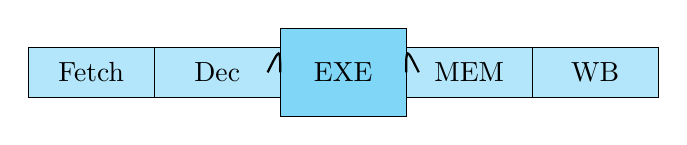
\begin{tikzpicture}[scale=0.8]
      % Single pipeline with bulge at EXE
      \draw[fill=cyan!30] (0,0) rectangle (2,0.8) node[midway] {Fetch};
      \draw[fill=cyan!30] (2,0) rectangle (4,0.8) node[midway] {Dec};
      \draw[fill=cyan!50] (4,-0.3) rectangle (6,1.1);
      \node at (5,0.4) {EXE};
      \draw[fill=cyan!30] (6,0) rectangle (8,0.8) node[midway] {MEM};
      \draw[fill=cyan!30] (8,0) rectangle (10,0.8) node[midway] {WB};
      
      % Curved lines showing bottleneck
      \draw[thick] (3.8,0.4) .. controls (4,0.8) and (4,0.8) .. (4,0.4);
      \draw[thick] (6,0.4) .. controls (6,0.8) and (6,0.8) .. (6.2,0.4);
    \end{tikzpicture}
  \end{center}
  
  \vspace{0.3cm}
  \begin{itemize}
    \item \textbf{Getting IPC $> 1$ requires to fetch, decode, exe, and retire $>1$ instruction per clock:}
  \end{itemize}
  
  \begin{center}
    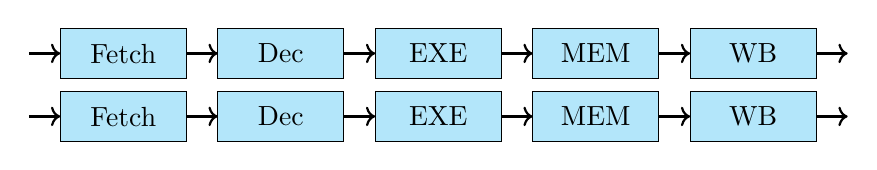
\begin{tikzpicture}[scale=0.8]
      % Dual pipeline
      \foreach \y in {0, -1} {
        \draw[->, thick] (-0.5,\y+0.4) -- (0,\y+0.4);
        \draw[fill=cyan!30] (0,\y) rectangle (2,\y+0.8) node[midway] {Fetch};
        \draw[->, thick] (2,\y+0.4) -- (2.5,\y+0.4);
        \draw[fill=cyan!30] (2.5,\y) rectangle (4.5,\y+0.8) node[midway] {Dec};
        \draw[->, thick] (4.5,\y+0.4) -- (5,\y+0.4);
        \draw[fill=cyan!30] (5,\y) rectangle (7,\y+0.8) node[midway] {EXE};
        \draw[->, thick] (7,\y+0.4) -- (7.5,\y+0.4);
        \draw[fill=cyan!30] (7.5,\y) rectangle (9.5,\y+0.8) node[midway] {MEM};
        \draw[->, thick] (9.5,\y+0.4) -- (10,\y+0.4);
        \draw[fill=cyan!30] (10,\y) rectangle (12,\y+0.8) node[midway] {WB};
        \draw[->, thick] (12,\y+0.4) -- (12.5,\y+0.4);
      }
    \end{tikzpicture}
  \end{center}
\end{frame}

\begin{frame}{The Pentium® Processor (1993)}
  \begin{itemize}
    \item \textbf{Fetch and decode 2 instructions per cycle}
    
    \item \textbf{At decode stage decide on \emph{pairing}:} can the two instructions be executed in parallel
    
    \item \textbf{Pairing decision is based on:}
    \begin{itemize}
      \item \textcolor{blue}{Data dependencies}: 2nd instruction must be independent of 1st
      \begin{itemize}
        \item If the 1st instruction produces data needed by the 2nd instruction, the 2nd instruction cannot be executed in parallel to the 1st instruction
      \end{itemize}
      
      \item \textcolor{blue}{Resources}: U-pipe and V-pipe are not symmetric (save HW)
      \begin{itemize}
        \item Common instructions can execute on either pipe
        \item Some instructions can execute only on the U-pipe
        \item V-pipe can run a subset of the instructions that can run on U-pipe
        \item If the 2nd instruction requires the U-pipe, it cannot pair
        \item Some instructions use resources of both pipes (and therefore cannot pair)
      \end{itemize}
    \end{itemize}
  \end{itemize}
  
  \begin{center}
    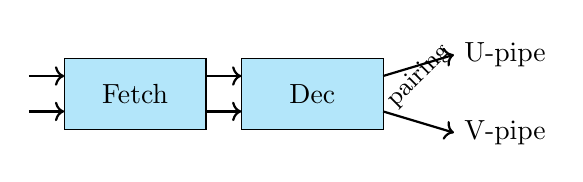
\begin{tikzpicture}[scale=0.9]
      \draw[->, thick] (-0.5,0) -- (0,0);
      \draw[->, thick] (-0.5,-0.5) -- (0,-0.5);
      \draw[fill=cyan!30] (0,-0.75) rectangle (2,0.25) node[midway] {Fetch};
      \draw[->, thick] (2,0) -- (2.5,0);
      \draw[->, thick] (2,-0.5) -- (2.5,-0.5);
      \draw[fill=cyan!30] (2.5,-0.75) rectangle (4.5,0.25) node[midway] {Dec};
      \node[rotate=45] at (5,0) {\small pairing};
      \draw[->, thick] (4.5,0) -- (5.5,0.3) node[right] {U-pipe};
      \draw[->, thick] (4.5,-0.5) -- (5.5,-0.8) node[right] {V-pipe};
    \end{tikzpicture}
  \end{center}
\end{frame}

\begin{frame}{Misprediction Penalty in a Superscalar CPU}
  \begin{itemize}
    \item \textbf{Assume}
    \begin{itemize}
      \item $\frac{1}{100}$ instruction is a mispredicted jump (MPI = 1\%)
      \item Flush penalty of 5 cycles
    \end{itemize}
    
    \vspace{0.5cm}
    
    \item \textbf{For IPC = 2}
    \begin{itemize}
      \item Flush every $\frac{100}{2} = 50$ cycles
      \item 5 cycles flush penalty every 50 cycles $\Rightarrow$ \alert{10\% performance hit}
    \end{itemize}
    
    \vspace{0.5cm}
    
    \item \textbf{For IPC = 1}
    \begin{itemize}
      \item Flush every $\frac{100}{1} = 100$ cycles
      \item 5 cycles flush penalty per 100 cycles $\Rightarrow$ \alert{5\% performance hit}
    \end{itemize}
    
    \vspace{0.5cm}
    
    \item \alert{Flush penalty increases as the machine is deeper and wider}
  \end{itemize}
\end{frame}

\begin{frame}{Extract More ILP}
  \begin{itemize}
    \item \textbf{ILP -- Instruction Level Parallelism}
    \begin{itemize}
      \item A given program, executed on a given input data has a given parallelism
      \item Can execute only independent instructions in parallel
      \item If for example each instruction is dependent on the previous instruction, ILP = 1
      \begin{itemize}
        \item Adding more HW will not change that
      \end{itemize}
    \end{itemize}
    
    \item \textbf{Adjacent instructions are usually dependent}
    \begin{itemize}
      \item 2nd pipe utilization is lower than 1st pipe utilization, a 3rd pipe utilization further goes down
    \end{itemize}
    
    \item \textbf{Cache misses stall execution} -- instructions dependent on a missed load stall
    
    \item \textbf{Compilers are limited to basic blocks}, and are not aware of cache misses
    
    \item \textbf{Solution: Out-Of-Order Execution}
    \begin{itemize}
      \item Look for independent instructions further ahead in the program
      \item Execute instructions based on data readiness
      \item Still need to keep the semantics of the original program
    \end{itemize}
  \end{itemize}
\end{frame}

\begin{frame}{Data Flow Analysis}
  \begin{columns}
    \begin{column}{0.35\textwidth}
      \textbf{Example:}
      \begin{enumerate}
        \item \texttt{\textcolor{r1color}{r1} $\leftarrow$ r4 / r7}
        \item \texttt{\textcolor{r8color}{r8} $\leftarrow$ \textcolor{r1color}{r1} + r2}
        \item \texttt{\textcolor{r5color}{r5} $\leftarrow$ r5 + 1}
        \item \texttt{\textcolor{r6color}{r6} $\leftarrow$ r6 - r3}
        \item \texttt{\textcolor{r4color}{r4} $\leftarrow$ \textcolor{r5color}{r5} + \textcolor{r6color}{r6}}
        \item \texttt{r7 $\leftarrow$ \textcolor{r8color}{r8} * \textcolor{r4color}{r4}}
      \end{enumerate}
      
      \vspace{0.3cm}
      \small{Assume divide takes multiple cycles}
    \end{column}
    
    \begin{column}{0.65\textwidth}
      \begin{center}
        \textbf{Data Flow Graph}\\
        \vspace{0.3cm}
        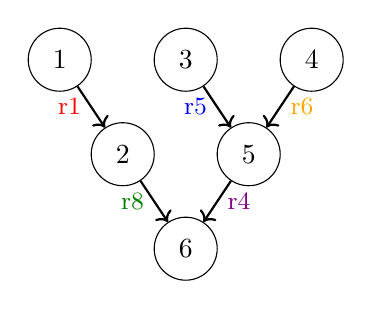
\begin{tikzpicture}[scale=0.8, 
          node distance=1.2cm,
          inst/.style={circle, draw, minimum size=0.8cm},
          dep/.style={->, thick}]
          
          % Nodes
          \node[inst] (i1) at (0,2.5) {1};
          \node[inst] (i3) at (2,2.5) {3};
          \node[inst] (i4) at (4,2.5) {4};
          \node[inst] (i2) at (1,1) {2};
          \node[inst] (i5) at (3,1) {5};
          \node[inst] (i6) at (2,-0.5) {6};
          
          % Dependencies with colored labels
          \draw[dep] (i1) -- node[left] {\textcolor{r1color}{\small r1}} (i2);
          \draw[dep] (i3) -- node[left] {\textcolor{r5color}{\small r5}} (i5);
          \draw[dep] (i4) -- node[right] {\textcolor{r6color}{\small r6}} (i5);
          \draw[dep] (i2) -- node[left] {\textcolor{r8color}{\small r8}} (i6);
          \draw[dep] (i5) -- node[right] {\textcolor{r4color}{\small r4}} (i6);
        \end{tikzpicture}
        
        \vspace{0.5cm}
        \small
        \begin{tabular}{cc}
          \textbf{In-order execution} & \textbf{Out-of-order execution} \\
        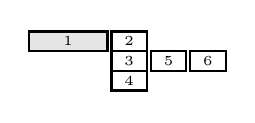
\begin{tikzpicture}[scale=0.5]
        % Box 1 (large, left side)
        \draw[thick, fill=gray!20] (0,1) rectangle (2,1.5) node[midway, font=\tiny] {1};
        
        % Box 2 (top right)
        \draw[thick, fill=white] (2.1,1) rectangle (3,1.5) node[midway, font=\tiny] {2};
        
        % Box 3 (middle right)
        \draw[thick, fill=white] (2.1,0.5) rectangle (3,1) node[midway, font=\tiny] {3};
        
        % Box 4 (bottom middle)
        \draw[thick, fill=white] (2.1,0) rectangle (3,0.5) node[midway, font=\tiny] {4};
        
        % Box 5 (right of box 3)
        \draw[thick, fill=white] (3.1,0.5) rectangle (4,1) node[midway, font=\tiny] {5};
        
        % Box 6 (far right)
        \draw[thick, fill=white] (4.1,0.5) rectangle (5,1) node[midway, font=\tiny] {6};
        \end{tikzpicture}
          &
          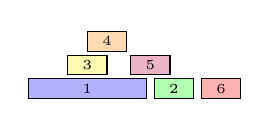
\begin{tikzpicture}[scale=0.5]
            \draw[fill=blue!30] (0,0) rectangle (3,0.5) node[midway] {\tiny 1};
            \draw[fill=yellow!30] (1,0.6) rectangle (2,1.1) node[midway] {\tiny 3};
            \draw[fill=orange!30] (1.5,1.2) rectangle (2.5,1.7) node[midway] {\tiny 4};
            \draw[fill=purple!30] (2.6,0.6) rectangle (3.6,1.1) node[midway] {\tiny 5};
            \draw[fill=green!30] (3.2,0) rectangle (4.2,0.5) node[midway] {\tiny 2};
            \draw[fill=red!30] (4.4,0) rectangle (5.4,0.5) node[midway] {\tiny 6};
          \end{tikzpicture}
        \end{tabular}
      \end{center}
    \end{column}
  \end{columns}
\end{frame}

\begin{frame}{OOOE -- General Scheme}
  \begin{center}
    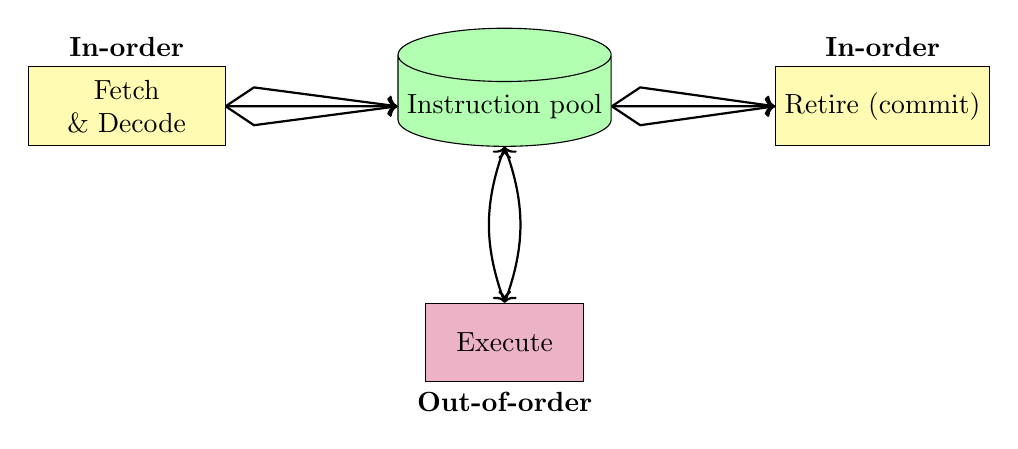
\begin{tikzpicture}[scale=1.2,
      block/.style={rectangle, draw, fill=yellow!30, minimum width=2.5cm, minimum height=1cm},
      pool/.style={cylinder, draw, fill=green!30, minimum width=2cm, minimum height=1.5cm, shape border rotate=90, aspect=0.25},
      exe/.style={rectangle, draw, fill=purple!30, minimum width=2cm, minimum height=1cm}]
      
      % Blocks
      \node[block,align=center] (fetch) at (0,0) {Fetch \\\& Decode};
      \node[pool] (pool) at (4,0) {Instruction pool};
      \node[exe] (exec) at (4,-2.5) {Execute};
      \node[block] (retire) at (8,0) {Retire (commit)};
      
      % Arrows with multiple lines
      \foreach \y in {-0.2, 0, 0.2} {
        \draw[->, thick] (fetch.east) -- ++(0.3,\y) -- (pool.west);
        \draw[->, thick] (pool.east) -- ++(0.3,\y) -- (retire.west);
      }
      
      % Bidirectional connection pool-execute
      \draw[<->, thick, bend right=20] (pool.south) to (exec.north);
      \draw[<->, thick, bend left=20] (pool.south) to (exec.north);
      
      % Labels
      \node[above] at (fetch.north) {\textbf{In-order}};
      \node[above] at (retire.north) {\textbf{In-order}};
      \node[below] at (exec.south) {\textbf{Out-of-order}};
    \end{tikzpicture}
  \end{center}
  
  \vspace{0.5cm}
  
  \begin{itemize}
    \item \textbf{Fetch \& decode instructions in parallel but in-order}
    \begin{itemize}
      \item Fill the Instruction Pool
    \end{itemize}
    
    \item \textbf{Execute ready instructions from the instructions pool}
    \begin{itemize}
      \item All source data ready + needed execution resources available
    \end{itemize}
    
    \item \textbf{Once an instruction is executed}
    \begin{itemize}
      \item Signal all dependent instructions that data is ready
    \end{itemize}
    
    \item \textbf{Commit instructions in parallel but in-order}
    \begin{itemize}
      \item State change (memory, register) and fault/exception handling
    \end{itemize}
  \end{itemize}
\end{frame}

\begin{frame}{Write-After-Write Dependency}
  \begin{columns}
    \begin{column}{0.5\textwidth}
      \textbf{Example Code:} \\
      \begin{tabular}{lll}
        (1) & & \texttt{\textcolor{r1color}{r1} $\leftarrow$ r9/17} \\
        (2) & & \texttt{\textcolor{r2color}{r2} $\leftarrow$ \textcolor{r2color}{r2}+\textcolor{r1color}{r1}} \\
        (3) & & \texttt{\textcolor{orange}{r1} $\leftarrow$ 23} \\
        (4) & & \texttt{\textcolor{r3color}{r3} $\leftarrow$ \textcolor{r3color}{r3}+\textcolor{orange}{r1}} \\
        (5) & & \texttt{jcc L2} \\
        (6) & \texttt{L2:} & \texttt{\textcolor{green}{r1} $\leftarrow$ 35} \\
        (7) & & \texttt{\textcolor{r4color}{r4} $\leftarrow$ \textcolor{r3color}{r3}+\textcolor{green}{r1}} \\
        (8) & & \texttt{\textcolor{blue}{r3} $\leftarrow$ 2} \\
      \end{tabular}
    \end{column}
    
    \begin{column}{0.5\textwidth}
      \begin{block}{WAW Issue}
        If inst (3) is executed before inst (1), r1 ends up having a wrong value.
        
        \vspace{0.3cm}
        
        Called \alert{write-after-write false dependency}:
        
        The order of two writes to the same register is flipped.
      \end{block}
    \end{column}
  \end{columns}
\end{frame}
\begin{frame}{What's Next}
  \begin{itemize}
    \item \textbf{Goal: minimize CPU Time}
    \begin{equation*}
      \text{CPU Time} = \text{clock cycle} \times \text{CPI} \times \text{IC}
    \end{equation*}
    
    \item \textbf{So far we have learned}
    \begin{itemize}
      \item Minimize clock cycle $\Rightarrow$ add more pipe stages
      \item Minimize CPI $\Rightarrow$ use pipeline
      \item Minimize IC $\Rightarrow$ architecture
    \end{itemize}
    
    \item \textbf{In a pipelined CPU}
    \begin{itemize}
      \item CPI w/o hazards is 1
      \item CPI with hazards is $> 1$
    \end{itemize}
    
    \item \textbf{Adding more pipe stages reduces clock cycle but increases CPI}
    \begin{itemize}
      \item Higher penalty due to control hazards
      \item More data hazards
    \end{itemize}
    
    \item \alert{What can we do? Further reduce the CPI!}
  \end{itemize}
\end{frame}

\begin{frame}{A Superscalar CPU}
  \begin{itemize}
    \item \textbf{Duplicating HW in one pipe stage won't help}
    \begin{itemize}
      \item e.g., have 2 ALUs
      \item the bottleneck moves to other stages
    \end{itemize}
  \end{itemize}
  
  \begin{center}
    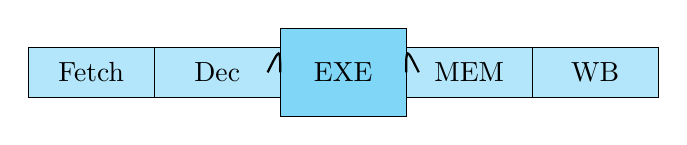
\begin{tikzpicture}[scale=0.8]
      % Single pipeline with bulge at EXE
      \draw[fill=cyan!30] (0,0) rectangle (2,0.8) node[midway] {Fetch};
      \draw[fill=cyan!30] (2,0) rectangle (4,0.8) node[midway] {Dec};
      \draw[fill=cyan!50] (4,-0.3) rectangle (6,1.1);
      \node at (5,0.4) {EXE};
      \draw[fill=cyan!30] (6,0) rectangle (8,0.8) node[midway] {MEM};
      \draw[fill=cyan!30] (8,0) rectangle (10,0.8) node[midway] {WB};
      
      % Curved lines showing bottleneck
      \draw[thick] (3.8,0.4) .. controls (4,0.8) and (4,0.8) .. (4,0.4);
      \draw[thick] (6,0.4) .. controls (6,0.8) and (6,0.8) .. (6.2,0.4);
    \end{tikzpicture}
  \end{center}
  
  \vspace{0.3cm}
  \begin{itemize}
    \item \textbf{Getting IPC $> 1$ requires to fetch, decode, exe, and retire $>1$ instruction per clock:}
  \end{itemize}
  
  \begin{center}
    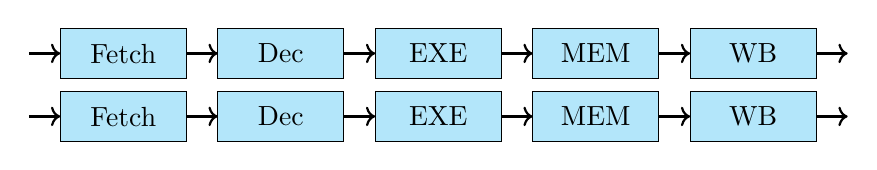
\begin{tikzpicture}[scale=0.8]
      % Dual pipeline
      \foreach \y in {0, -1} {
        \draw[->, thick] (-0.5,\y+0.4) -- (0,\y+0.4);
        \draw[fill=cyan!30] (0,\y) rectangle (2,\y+0.8) node[midway] {Fetch};
        \draw[->, thick] (2,\y+0.4) -- (2.5,\y+0.4);
        \draw[fill=cyan!30] (2.5,\y) rectangle (4.5,\y+0.8) node[midway] {Dec};
        \draw[->, thick] (4.5,\y+0.4) -- (5,\y+0.4);
        \draw[fill=cyan!30] (5,\y) rectangle (7,\y+0.8) node[midway] {EXE};
        \draw[->, thick] (7,\y+0.4) -- (7.5,\y+0.4);
        \draw[fill=cyan!30] (7.5,\y) rectangle (9.5,\y+0.8) node[midway] {MEM};
        \draw[->, thick] (9.5,\y+0.4) -- (10,\y+0.4);
        \draw[fill=cyan!30] (10,\y) rectangle (12,\y+0.8) node[midway] {WB};
        \draw[->, thick] (12,\y+0.4) -- (12.5,\y+0.4);
      }
    \end{tikzpicture}
  \end{center}
\end{frame}

\begin{frame}{The Pentium® Processor (1993)}
  \begin{itemize}
    \item \textbf{Fetch and decode 2 instructions per cycle}
    
    \item \textbf{At decode stage decide on \emph{pairing}:} can the two instructions be executed in parallel
    
    \item \textbf{Pairing decision is based on:}
    \begin{itemize}
      \item \textcolor{blue}{Data dependencies}: 2nd instruction must be independent of 1st
      \begin{itemize}
        \item If the 1st instruction produces data needed by the 2nd instruction, the 2nd instruction cannot be executed in parallel to the 1st instruction
      \end{itemize}
      
      \item \textcolor{blue}{Resources}: U-pipe and V-pipe are not symmetric (save HW)
      \begin{itemize}
        \item Common instructions can execute on either pipe
        \item Some instructions can execute only on the U-pipe
        \item V-pipe can run a subset of the instructions that can run on U-pipe
        \item If the 2nd instruction requires the U-pipe, it cannot pair
        \item Some instructions use resources of both pipes (and therefore cannot pair)
      \end{itemize}
    \end{itemize}
  \end{itemize}
  
  \begin{center}
    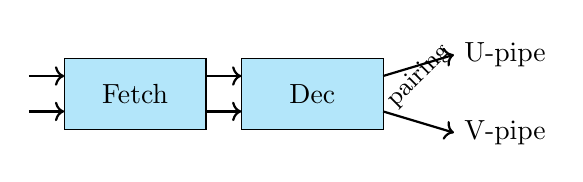
\begin{tikzpicture}[scale=0.9]
      \draw[->, thick] (-0.5,0) -- (0,0);
      \draw[->, thick] (-0.5,-0.5) -- (0,-0.5);
      \draw[fill=cyan!30] (0,-0.75) rectangle (2,0.25) node[midway] {Fetch};
      \draw[->, thick] (2,0) -- (2.5,0);
      \draw[->, thick] (2,-0.5) -- (2.5,-0.5);
      \draw[fill=cyan!30] (2.5,-0.75) rectangle (4.5,0.25) node[midway] {Dec};
      \node[rotate=45] at (5,0) {\small pairing};
      \draw[->, thick] (4.5,0) -- (5.5,0.3) node[right] {U-pipe};
      \draw[->, thick] (4.5,-0.5) -- (5.5,-0.8) node[right] {V-pipe};
    \end{tikzpicture}
  \end{center}
\end{frame}

\begin{frame}{Misprediction Penalty in a Superscalar CPU}
  \begin{itemize}
    \item \textbf{Assume}
    \begin{itemize}
      \item $\frac{1}{100}$ instruction is a mispredicted jump (MPI = 1\%)
      \item Flush penalty of 5 cycles
    \end{itemize}
    
    \vspace{0.5cm}
    
    \item \textbf{For IPC = 2}
    \begin{itemize}
      \item Flush every $\frac{100}{2} = 50$ cycles
      \item 5 cycles flush penalty every 50 cycles $\Rightarrow$ \alert{10\% performance hit}
    \end{itemize}
    
    \vspace{0.5cm}
    
    \item \textbf{For IPC = 1}
    \begin{itemize}
      \item Flush every $\frac{100}{1} = 100$ cycles
      \item 5 cycles flush penalty per 100 cycles $\Rightarrow$ \alert{5\% performance hit}
    \end{itemize}
    
    \vspace{0.5cm}
    
    \item \alert{Flush penalty increases as the machine is deeper and wider}
  \end{itemize}
\end{frame}

\begin{frame}{Extract More ILP}
  \begin{itemize}
    \item \textbf{ILP -- Instruction Level Parallelism}
    \begin{itemize}
      \item A given program, executed on a given input data has a given parallelism
      \item Can execute only independent instructions in parallel
      \item If for example each instruction is dependent on the previous instruction, ILP = 1
      \begin{itemize}
        \item Adding more HW will not change that
      \end{itemize}
    \end{itemize}
    
    \item \textbf{Adjacent instructions are usually dependent}
    \begin{itemize}
      \item 2nd pipe utilization is lower than 1st pipe utilization, a 3rd pipe utilization further goes down
    \end{itemize}
    
    \item \textbf{Cache misses stall execution} -- instructions dependent on a missed load stall
    
    \item \textbf{Compilers are limited to basic blocks}, and are not aware of cache misses
    
    \item \textbf{Solution: Out-Of-Order Execution}
    \begin{itemize}
      \item Look for independent instructions further ahead in the program
      \item Execute instructions based on data readiness
      \item Still need to keep the semantics of the original program
    \end{itemize}
  \end{itemize}
\end{frame}

\begin{frame}{Data Flow Analysis}
  \begin{columns}
    \begin{column}{0.35\textwidth}
      \textbf{Example:}
      \begin{enumerate}
        \item \texttt{\textcolor{r1color}{r1} $\leftarrow$ r4 / r7}
        \item \texttt{\textcolor{r8color}{r8} $\leftarrow$ \textcolor{r1color}{r1} + r2}
        \item \texttt{\textcolor{r5color}{r5} $\leftarrow$ r5 + 1}
        \item \texttt{\textcolor{r6color}{r6} $\leftarrow$ r6 - r3}
        \item \texttt{\textcolor{r4color}{r4} $\leftarrow$ \textcolor{r5color}{r5} + \textcolor{r6color}{r6}}
        \item \texttt{r7 $\leftarrow$ \textcolor{r8color}{r8} * \textcolor{r4color}{r4}}
      \end{enumerate}
      
      \vspace{0.3cm}
      \small{Assume divide takes multiple cycles}
    \end{column}
    
    \begin{column}{0.65\textwidth}
      \begin{center}
        \textbf{Data Flow Graph}\\
        \vspace{0.3cm}
        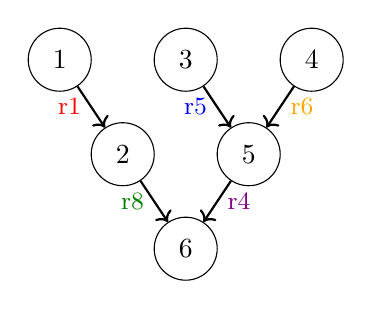
\begin{tikzpicture}[scale=0.8, 
          node distance=1.2cm,
          inst/.style={circle, draw, minimum size=0.8cm},
          dep/.style={->, thick}]
          
          % Nodes
          \node[inst] (i1) at (0,2.5) {1};
          \node[inst] (i3) at (2,2.5) {3};
          \node[inst] (i4) at (4,2.5) {4};
          \node[inst] (i2) at (1,1) {2};
          \node[inst] (i5) at (3,1) {5};
          \node[inst] (i6) at (2,-0.5) {6};
          
          % Dependencies with colored labels
          \draw[dep] (i1) -- node[left] {\textcolor{r1color}{\small r1}} (i2);
          \draw[dep] (i3) -- node[left] {\textcolor{r5color}{\small r5}} (i5);
          \draw[dep] (i4) -- node[right] {\textcolor{r6color}{\small r6}} (i5);
          \draw[dep] (i2) -- node[left] {\textcolor{r8color}{\small r8}} (i6);
          \draw[dep] (i5) -- node[right] {\textcolor{r4color}{\small r4}} (i6);
        \end{tikzpicture}
        
        \vspace{0.5cm}
        \small
        \begin{tabular}{cc}
          \textbf{In-order execution} & \textbf{Out-of-order execution} \\
        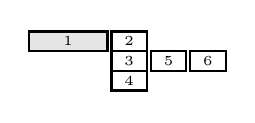
\begin{tikzpicture}[scale=0.5]
        % Box 1 (large, left side)
        \draw[thick, fill=gray!20] (0,1) rectangle (2,1.5) node[midway, font=\tiny] {1};
        
        % Box 2 (top right)
        \draw[thick, fill=white] (2.1,1) rectangle (3,1.5) node[midway, font=\tiny] {2};
        
        % Box 3 (middle right)
        \draw[thick, fill=white] (2.1,0.5) rectangle (3,1) node[midway, font=\tiny] {3};
        
        % Box 4 (bottom middle)
        \draw[thick, fill=white] (2.1,0) rectangle (3,0.5) node[midway, font=\tiny] {4};
        
        % Box 5 (right of box 3)
        \draw[thick, fill=white] (3.1,0.5) rectangle (4,1) node[midway, font=\tiny] {5};
        
        % Box 6 (far right)
        \draw[thick, fill=white] (4.1,0.5) rectangle (5,1) node[midway, font=\tiny] {6};
        \end{tikzpicture}
          &
          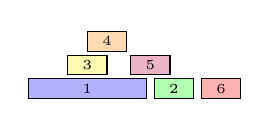
\begin{tikzpicture}[scale=0.5]
            \draw[fill=blue!30] (0,0) rectangle (3,0.5) node[midway] {\tiny 1};
            \draw[fill=yellow!30] (1,0.6) rectangle (2,1.1) node[midway] {\tiny 3};
            \draw[fill=orange!30] (1.5,1.2) rectangle (2.5,1.7) node[midway] {\tiny 4};
            \draw[fill=purple!30] (2.6,0.6) rectangle (3.6,1.1) node[midway] {\tiny 5};
            \draw[fill=green!30] (3.2,0) rectangle (4.2,0.5) node[midway] {\tiny 2};
            \draw[fill=red!30] (4.4,0) rectangle (5.4,0.5) node[midway] {\tiny 6};
          \end{tikzpicture}
        \end{tabular}
      \end{center}
    \end{column}
  \end{columns}
\end{frame}

\begin{frame}{OOOE -- General Scheme}
  \begin{center}
    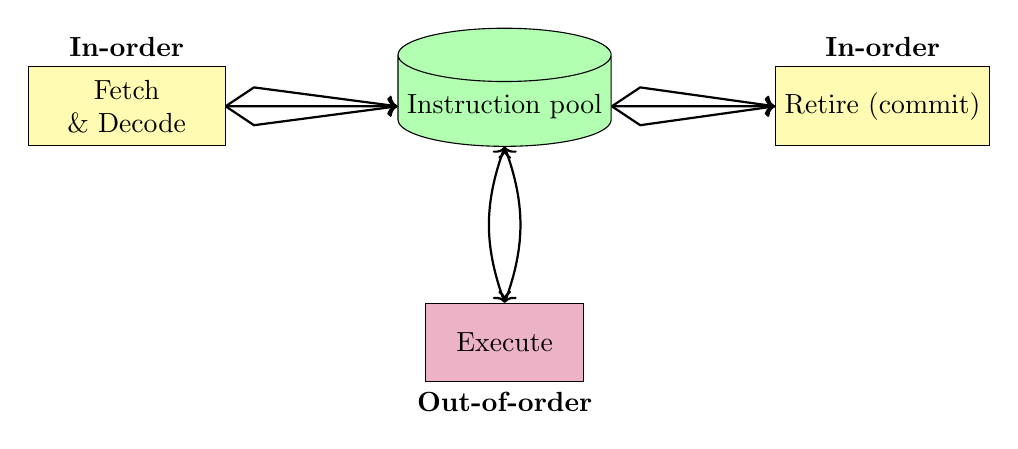
\begin{tikzpicture}[scale=1.2,
      block/.style={rectangle, draw, fill=yellow!30, minimum width=2.5cm, minimum height=1cm},
      pool/.style={cylinder, draw, fill=green!30, minimum width=2cm, minimum height=1.5cm, shape border rotate=90, aspect=0.25},
      exe/.style={rectangle, draw, fill=purple!30, minimum width=2cm, minimum height=1cm}]
      
      % Blocks
      \node[block,align=center] (fetch) at (0,0) {Fetch \\\& Decode};
      \node[pool] (pool) at (4,0) {Instruction pool};
      \node[exe] (exec) at (4,-2.5) {Execute};
      \node[block] (retire) at (8,0) {Retire (commit)};
      
      % Arrows with multiple lines
      \foreach \y in {-0.2, 0, 0.2} {
        \draw[->, thick] (fetch.east) -- ++(0.3,\y) -- (pool.west);
        \draw[->, thick] (pool.east) -- ++(0.3,\y) -- (retire.west);
      }
      
      % Bidirectional connection pool-execute
      \draw[<->, thick, bend right=20] (pool.south) to (exec.north);
      \draw[<->, thick, bend left=20] (pool.south) to (exec.north);
      
      % Labels
      \node[above] at (fetch.north) {\textbf{In-order}};
      \node[above] at (retire.north) {\textbf{In-order}};
      \node[below] at (exec.south) {\textbf{Out-of-order}};
    \end{tikzpicture}
  \end{center}
  
  \vspace{0.5cm}
  
  \begin{itemize}
    \item \textbf{Fetch \& decode instructions in parallel but in-order}
    \begin{itemize}
      \item Fill the Instruction Pool
    \end{itemize}
    
    \item \textbf{Execute ready instructions from the instructions pool}
    \begin{itemize}
      \item All source data ready + needed execution resources available
    \end{itemize}
    
    \item \textbf{Once an instruction is executed}
    \begin{itemize}
      \item Signal all dependent instructions that data is ready
    \end{itemize}
    
    \item \textbf{Commit instructions in parallel but in-order}
    \begin{itemize}
      \item State change (memory, register) and fault/exception handling
    \end{itemize}
  \end{itemize}
\end{frame}

\begin{frame}{Write-After-Write Dependency}
  \begin{columns}
    \begin{column}{0.5\textwidth}
      \textbf{Example Code:} \\
      \begin{tabular}{lll}
        (1) & & \texttt{\textcolor{blue}{r1} $\leftarrow$ r9/17} \\
        (2) & & \texttt{r2 $\leftarrow$ r2+\textcolor{blue}{r1}} \\
        (3) & & \texttt{\textcolor{orange}{r1} $\leftarrow$ 23} \\
        (4) & & \texttt{r3 $\leftarrow$ r3+\textcolor{orange}{r1}} \\
        (5) & & \texttt{jcc L2} \\
        (6) & \texttt{L2:} & \texttt{\textcolor{green}{r1} $\leftarrow$ 35} \\
        (7) & & \texttt{r4 $\leftarrow$ r3+\textcolor{green}{r1}} \\
        (8) & & \texttt{r3 $\leftarrow$ 2} \\
      \end{tabular}
    \end{column}
    
    \begin{column}{0.5\textwidth}
      \begin{block}{WAW Issue}
        If inst (3) is executed before inst (1), r1 ends up having a wrong value.
        
        \vspace{0.3cm}
        
        Called \alert{write-after-write false dependency}:
        
        The order of two writes to the same register is flipped.
      \end{block}
    \end{column}
  \end{columns}
\end{frame}

\begin{frame}{Write-After-Write Dependency}
  \begin{columns}
    \begin{column}{0.5\textwidth}
      \textbf{Example Code (reordered):} \\
      \begin{tabular}{lll}
        (3) & & \texttt{\textcolor{orange}{r1} $\leftarrow$ 23} \\
        (1) & & \texttt{\textcolor{blue}{r1} $\leftarrow$ r9/17} \\
        (2) & & \texttt{r2 $\leftarrow$ r2+\textcolor{blue}{r1}} \\
        & & \\
        (4) & & \texttt{r3 $\leftarrow$ r3+\textcolor{orange}{r1}} \\
        (5) & & \texttt{jcc L2} \\
        (6) & \texttt{L2:} & \texttt{\textcolor{green}{r1} $\leftarrow$ 35} \\
        (7) & & \texttt{r4 $\leftarrow$ r3+\textcolor{green}{r1}} \\
        (8) & & \texttt{r3 $\leftarrow$ 2} \\
      \end{tabular}
    \end{column}
    
    \begin{column}{0.5\textwidth}
      \begin{block}{Correct Dependency}
        Inst (4) should use the value of \textcolor{orange}{r1} produced by inst (3), even if inst (1) is executed after inst (3).
        
        \vspace{0.3cm}
        
        \alert{Write-After-Write (WAW) is a \emph{false dependency}}
        
        Not a real data dependency, but an artifact of OOO execution
      \end{block}
      
      % Arrow showing dependency
      \begin{tikzpicture}[overlay, remember picture]
        \draw[->, thick, orange, dashed] (-4.5,1.8) -- (-2.8,0.8);
      \end{tikzpicture}
    \end{column}
  \end{columns}
\end{frame}

\begin{frame}{Speculative Execution}
  \begin{columns}
    \begin{column}{0.45\textwidth}
      \textbf{Example Code:} \\
      \begin{tabular}{lll}
        (3) & & \texttt{\textcolor{orange}{r1} $\leftarrow$ 23} \\
        (1) & & \texttt{\textcolor{blue}{r1} $\leftarrow$ r9/17} \\
        (2) & & \texttt{r2 $\leftarrow$ r2+\textcolor{blue}{r1}} \\
        (4) & & \texttt{r3 $\leftarrow$ r3+\textcolor{orange}{r1}} \\
        (5) & & \texttt{jcc L2} \\
        \rowcolor{pink!30} (6) & \texttt{L2:} & \texttt{\textcolor{green}{r1} $\leftarrow$ 35} \\
        \rowcolor{pink!30} (7) & & \texttt{r4 $\leftarrow$ r3+\textcolor{green}{r1}} \\
        \rowcolor{pink!30} (8) & & \texttt{r3 $\leftarrow$ 2} \\
      \end{tabular}
    \end{column}
    
    \begin{column}{0.55\textwidth}
      \begin{block}{OOO Speculative Execution}
        \small
        \textbf{Every 5th instruction is a branch} $\Rightarrow$ must continue fetching along \textcolor{green}{predicted path} to fill instruction pool.
        
        Without speculation: limited to finding independent instructions only until next branch.
        
        \alert{Speculative Execution:} Execute instructions from predicted path before branch resolution.
        
        Example: inst (6) can execute before inst (1).
        
        If mispredicted: must undo speculatively executed instructions.
      \end{block}
    \end{column}
  \end{columns}
\end{frame}

\begin{frame}{Write-After-Read Dependency}
  \begin{columns}
    \begin{column}{0.5\textwidth}
      \textbf{Example Code:} \\
      \begin{tabular}{lll}
        (3) & & \texttt{\textcolor{orange}{r1} $\leftarrow$ 23} \\
        (1) & & \texttt{\textcolor{blue}{r1} $\leftarrow$ r9/17} \\
        (2) & & \texttt{r2 $\leftarrow$ r2+\textcolor{blue}{r1}} \\
        & & \\
        (4) & & \texttt{r3 $\leftarrow$ r3+\textcolor{orange}{r1}} \\
        (5) & & \texttt{jcc L2} \\
        (6) & \texttt{L2:} & \texttt{\textcolor{green}{r1} $\leftarrow$ 35} \\
        (8) & & \texttt{\textcolor{blue}{r3} $\leftarrow$ 2} \\
        (7) & & \texttt{r4 $\leftarrow$ \textcolor{red}{r3}+\textcolor{green}{r1}} \\
      \end{tabular}
    \end{column}
    
    \begin{column}{0.5\textwidth}
      \begin{block}{WAR Issue}
        If inst (8) is executed before inst (7), inst (7) gets a wrong value of r3.
        
        \vspace{0.3cm}
        
        Called \alert{write-after-read false dependency}.
        
        \vspace{0.3cm}
        
        \alert{Write-After-Read (WAR) is a \emph{false dependency}}
        
        Not a real data dependency, but an artifact of OOO execution
      \end{block}
      
      % Arrow showing dependency
      \begin{tikzpicture}[overlay, remember picture]
        \draw[->, thick, red, dashed] (-2.5,-0.4) -- (-4,-1.2);
      \end{tikzpicture}
    \end{column}
  \end{columns}
\end{frame}

\begin{frame}{Register Renaming}
  \begin{itemize}
    \item \textbf{Physical register pool:} Maps architectural registers to physical registers
    
    \item \textbf{Allocation (in-order):}
    \begin{enumerate}
      \item If instruction writes Rx $\rightarrow$ allocate free physical register PRi
      \item Update mapping: Rx $\mapsto$ PRi
      \item Rename sources to their mapped physical registers
    \end{enumerate}
    
    \item \textbf{Execution (out-of-order):}
    \begin{itemize}
      \item Execute when sources ready \& resources available
      \item Write result to PRi (not Rx)
    \end{itemize}
    
    \item \textbf{Commit (in-order):}
    \begin{itemize}
      \item Copy PRi $\rightarrow$ Rx
      \item If Rx still maps to PRi: set mapping to architectural
      \item Return PRi to free pool
    \end{itemize}
  \end{itemize}
\end{frame}

\begin{frame}{Register Renaming}
  \begin{columns}
    \begin{column}{0.5\textwidth}
      \begin{tabular}{lll}
        \multicolumn{3}{c}{\textbf{Original}} \\
        (1) & r1 $\leftarrow$ 17 & \\
        (2) & r2 $\leftarrow$ r2+r1 & \\
        (3) & r1 $\leftarrow$ 23 & \\
        (4) & r3 $\leftarrow$ r3+r1 & \\
        (5) & jcc L2 & \\
        (6) L2: & r1 $\leftarrow$ 35 & \\
        (7) & r4 $\leftarrow$ r3+r1 & \\
        (8) & r3 $\leftarrow$ 2 & \\
      \end{tabular}
    \end{column}
    
    \begin{column}{0.5\textwidth}
      \begin{tabular}{lll}
        \multicolumn{3}{c}{\textbf{Renaming}} \\
        r1:pr1 & pr1 $\leftarrow$ 17 & \\
        r2:pr2 & pr2 $\leftarrow$ r2+pr1 & \\
        & & \\
        & & \\
        & & \\
        & & \\
        & & \\
        & & \\
      \end{tabular}
      
      \vspace{0.5cm}
      \begin{block}{Note}
        \small
        r2 is used for both source and destination.
        This explains why first the source registers are renamed according to the current mapping, and only then the mapping of the destination register r2 is updated by the newly allocated physical register pr2.
      \end{block}
    \end{column}
  \end{columns}
  
  \vspace{0.3cm}
  \begin{center}
    \begin{tabular}{|c|c|c|c|c|}
      \hline
      & r1 & r2 & r3 & r4 \\
      \hline
      Register mapping & pr1 & pr2 & r3 & r4 \\
      \hline
    \end{tabular}
  \end{center}
\end{frame}

\begin{frame}{Register Renaming}
  \begin{columns}
    \begin{column}{0.5\textwidth}
      \begin{tabular}{lll}
        \multicolumn{3}{c}{\textbf{Original}} \\
        (1) & r1 $\leftarrow$ 17 & \\
        (2) & r2 $\leftarrow$ r2+r1 & \\
        (3) & r1 $\leftarrow$ 23 & \\
        (4) & r3 $\leftarrow$ r3+r1 & \\
        (5) & jcc L2 & \\
        (6) L2: & r1 $\leftarrow$ 35 & \\
        (7) & r4 $\leftarrow$ r3+r1 & \\
        (8) & r3 $\leftarrow$ 2 & \\
      \end{tabular}
    \end{column}
    
    \begin{column}{0.5\textwidth}
      \begin{tabular}{lll}
        \multicolumn{3}{c}{\textbf{Renaming}} \\
        r1:pr1 & pr1 $\leftarrow$ 17 & \\
        r2:pr2 & pr2 $\leftarrow$ r2+pr1 & \\
        r1:pr3 & pr3 $\leftarrow$ 23 & \\
        r3:pr4 & pr4 $\leftarrow$ r3+pr3 & \\
        & & \\
        & & \\
        & & \\
        & & \\
      \end{tabular}
    \end{column}
  \end{columns}
  
  \vspace{0.5cm}
  \begin{center}
    \begin{tabular}{|c|c|c|c|c|}
      \hline
      & r1 & r2 & r3 & r4 \\
      \hline
      Register mapping & pr3 & pr2 & pr4 & r4 \\
      \hline
    \end{tabular}
  \end{center}
  
  \begin{center}
    \colorbox{green!30}{Each instruction uses the correct sources, regardless of the execution order}
  \end{center}
\end{frame}

\begin{frame}{Register Renaming}
  \begin{columns}
    \begin{column}{0.5\textwidth}
      \begin{tabular}{lll}
        \multicolumn{3}{c}{\textbf{Original}} \\
        (1) & r1 $\leftarrow$ 17 & \\
        (2) & r2 $\leftarrow$ r2+r1 & \\
        (3) & r1 $\leftarrow$ 23 & \\
        (4) & r3 $\leftarrow$ r3+r1 & \\
        (5) & jcc L2 & \\
        (6) L2: & r1 $\leftarrow$ 35 & \\
        (7) & r4 $\leftarrow$ r3+r1 & \\
        (8) & r3 $\leftarrow$ 2 & \\
      \end{tabular}
    \end{column}
    
    \begin{column}{0.5\textwidth}
      \begin{tabular}{lll}
        \multicolumn{3}{c}{\textbf{Renaming}} \\
        r1:pr1 & pr1 $\leftarrow$ 17 & \\
        r2:pr2 & pr2 $\leftarrow$ r2+pr1 & \\
        r1:pr3 & pr3 $\leftarrow$ 23 & \\
        r3:pr4 & pr4 $\leftarrow$ r3+pr3 & \\
        & & \\
        r1:pr5 & pr5 $\leftarrow$ 35 & \\
        r4:pr6 & pr6 $\leftarrow$ pr4+pr5 & \\
        r3:pr7 & pr7 $\leftarrow$ 2 & \\
      \end{tabular}
    \end{column}
  \end{columns}
  
  \vspace{0.5cm}
  \begin{center}
    \begin{tabular}{|c|c|c|c|c|}
      \hline
      & r1 & r2 & r3 & r4 \\
      \hline
      Register mapping & pr5 & pr2 & pr7 & pr6 \\
      \hline
    \end{tabular}
  \end{center}
  
  \begin{center}
    \colorbox{green!30}{Each instruction uses the correct sources, regardless of the execution order}
  \end{center}
\end{frame}

\begin{frame}{Speculative Execution -- Misprediction}
  \begin{columns}
    \begin{column}{0.5\textwidth}
      \begin{tabular}{lll}
        \multicolumn{3}{c}{\textbf{Original}} \\
        (1) & r1 $\leftarrow$ 17 & \\
        (2) & r2 $\leftarrow$ r2+r1 & \\
        (3) & r1 $\leftarrow$ 23 & \\
        (4) & r3 $\leftarrow$ r3+r1 & \\
        (5) & jcc L2 & \\
        \rowcolor{pink!30} (6) L2: & r1 $\leftarrow$ 35 & \\
        \rowcolor{pink!30} (7) & r4 $\leftarrow$ r3+r1 & \\
        \rowcolor{pink!30} (8) & r3 $\leftarrow$ 2 & \\
      \end{tabular}
    \end{column}
    
    \begin{column}{0.5\textwidth}
      \begin{tabular}{lll}
        \multicolumn{3}{c}{\textbf{Renaming}} \\
        r1:pr1 & pr1 $\leftarrow$ 17 & \\
        r2:pr2 & pr2 $\leftarrow$ r2+pr1 & \\
        r1:pr3 & pr3 $\leftarrow$ 23 & \\
        r3:pr4 & pr4 $\leftarrow$ r3+pr3 & \\
        & & \\
        \rowcolor{pink!30} r1:pr5 & pr5 $\leftarrow$ 35 & \\
        \rowcolor{pink!30} r4:pr6 & pr6 $\leftarrow$ pr4+pr5 & \\
        \rowcolor{pink!30} r3:pr7 & pr7 $\leftarrow$ 2 & \\
      \end{tabular}
    \end{column}
  \end{columns}
  
  \vspace{0.3cm}
  \begin{center}
    \begin{tabular}{|c|c|c|c|c|}
      \hline
      & r1 & r2 & r3 & r4 \\
      \hline
      Register mapping & pr3 & pr2 & pr4 & r4 \\
      \hline
    \end{tabular}
  \end{center}
  
  \begin{block}{Misprediction Recovery}
    If the predicted branch path turns out to be wrong (when the branch is executed):
    The instructions following the branch are flushed \textbf{before they are committed}
    $\Rightarrow$ the architectural state is not changed
  \end{block}
\end{frame}

\begin{frame}{Speculative Execution -- Misprediction}
  \begin{columns}
    \begin{column}{0.5\textwidth}
      \begin{tabular}{lll}
        \multicolumn{3}{c}{\textbf{Original}} \\
        (1) & r1 $\leftarrow$ 17 & \\
        (2) & r2 $\leftarrow$ r2+r1 & \\
        (3) & r1 $\leftarrow$ 23 & \\
        (4) & r3 $\leftarrow$ r3+r1 & \\
        (5) & jcc L2 & \\
        \rowcolor{pink!30} (6) L2: & r1 $\leftarrow$ 35 & \\
        \rowcolor{pink!30} (7) & r4 $\leftarrow$ r3+r1 & \\
        \rowcolor{pink!30} (8) & r3 $\leftarrow$ 2 & \\
      \end{tabular}
    \end{column}
    
    \begin{column}{0.5\textwidth}
      \begin{tabular}{lll}
        \multicolumn{3}{c}{\textbf{Renaming}} \\
        r1:pr1 & pr1 $\leftarrow$ 17 & \\
        r2:pr2 & pr2 $\leftarrow$ r2+pr1 & \\
        r1:pr3 & pr3 $\leftarrow$ 23 & \\
        r3:pr4 & pr4 $\leftarrow$ r3+pr3 & \\
        & & \\
        \rowcolor{pink!30} r1:pr5 & pr5 $\leftarrow$ 35 & \\
        \rowcolor{pink!30} r4:pr6 & pr6 $\leftarrow$ pr4+pr5 & \\
        \rowcolor{pink!30} r3:pr7 & pr7 $\leftarrow$ 2 & \\
      \end{tabular}
    \end{column}
  \end{columns}
  
  \vspace{0.3cm}
  \begin{center}
    \begin{tabular}{|c|c|c|c|c|}
      \hline
      & r1 & r2 & r3 & r4 \\
      \hline
      Register mapping & \textcolor{red}{\textcircled{pr5}} & pr2 & \textcolor{red}{\textcircled{pr7}} & \textcolor{red}{\textcircled{pr6}} \\
      \hline
    \end{tabular}
  \end{center}
  
  \begin{block}{Recovery Challenge}
    But the register mapping was already wrongly updated by the wrong path instructions
    
    \vspace{0.2cm}
    \colorbox{green!30}{Later on we will see various schemes for recovering the mapping}
  \end{block}
\end{frame}

\begin{frame}{A Superscalar OOO Machine}
  \begin{center}
    \colorbox{gray!20}{\textbf{In-order}}
    
    \vspace{0.3cm}
    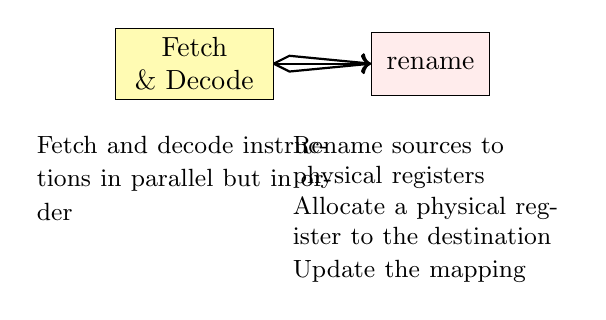
\begin{tikzpicture}[scale=1,
      block/.style={rectangle, draw, fill=yellow!30, minimum width=2cm, minimum height=0.8cm},
      rename/.style={rectangle, draw, fill=pink!30, minimum width=1.5cm, minimum height=0.8cm}]
      
      \node[block,align=center] (fetch) at (0,0) {Fetch \\\& Decode};
      \node[rename] (rename) at (3,0) {rename};
      
      % Multiple arrows from fetch to rename
      \foreach \y in {-0.1, 0, 0.1} {
        \draw[->, thick] (fetch.east) -- ++(0.2,\y) -- (rename.west);
      }
      
      % Annotations
      \node[text width=4cm, below] at (0,-0.8) {\small Fetch and decode instructions in parallel but in order};
      \node[text width=3.5cm, below] at (3,-0.8) {\small 
        Rename sources to physical registers\\
        Allocate a physical register to the destination\\
        Update the mapping};
    \end{tikzpicture}
  \end{center}
\end{frame}

\begin{frame}{A Superscalar OOO Machine}
  \begin{center}
    \colorbox{gray!20}{\textbf{In-order}}
    
    \vspace{0.3cm}
    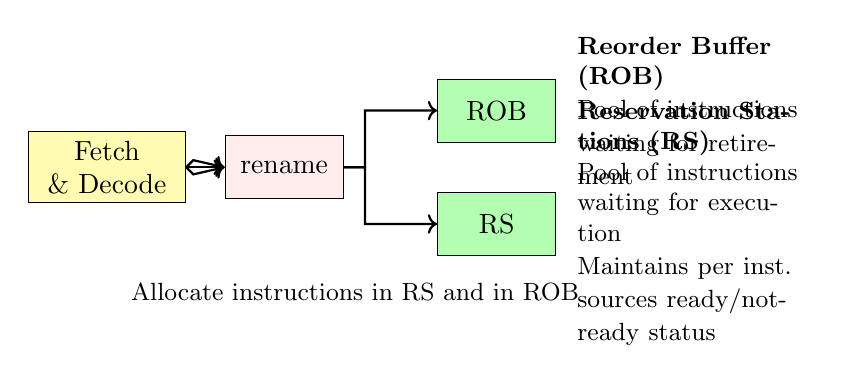
\begin{tikzpicture}[scale=0.9,
      block/.style={rectangle, draw, fill=yellow!30, minimum width=2cm, minimum height=0.8cm},
      rename/.style={rectangle, draw, fill=pink!30, minimum width=1.5cm, minimum height=0.8cm},
      pool/.style={rectangle, draw, fill=green!30, minimum width=1.5cm, minimum height=0.8cm}]
      
      \node[block,align=center] (fetch) at (0,0) {Fetch \\\& Decode};
      \node[rename] (rename) at (2.5,0) {rename};
      \node[pool] (rob) at (5.5,0.8) {ROB};
      \node[pool] (rs) at (5.5,-0.8) {RS};
      
      % Arrows
      \foreach \y in {-0.1, 0, 0.1} {
        \draw[->, thick] (fetch.east) -- ++(0.1,\y) -- (rename.west);
      }
      
      \draw[->, thick] (rename.east) -- ++(0.3,0) -- ++(0,0.8) -- (rob.west);
      \draw[->, thick] (rename.east) -- ++(0.3,0) -- ++(0,-0.8) -- (rs.west);
      
      % Annotations
      \node[text width=3cm, right] at (6.5,0.8) {\small \textbf{Reorder Buffer (ROB)} \\ Pool of instructions waiting for retirement};
      \node[text width=3cm, right] at (6.5,-0.8) {\small \textbf{Reservation Stations (RS)} \\ Pool of instructions waiting for execution \\ Maintains per inst. sources ready/not-ready status};
      
      \node[below] at (3.5,-1.5) {\small Allocate instructions in RS and in ROB};
    \end{tikzpicture}
  \end{center}
\end{frame}

\begin{frame}{A Superscalar OOO Machine}
  \begin{center}
    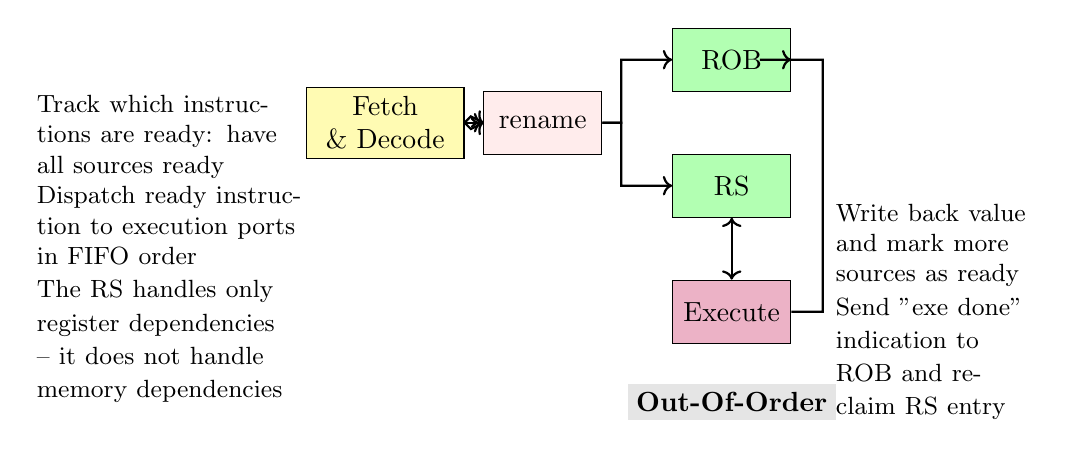
\begin{tikzpicture}[scale=0.8,
      block/.style={rectangle, draw, fill=yellow!30, minimum width=2cm, minimum height=0.8cm},
      rename/.style={rectangle, draw, fill=pink!30, minimum width=1.5cm, minimum height=0.8cm},
      pool/.style={rectangle, draw, fill=green!30, minimum width=1.5cm, minimum height=0.8cm},
      exe/.style={rectangle, draw, fill=purple!30, minimum width=1.5cm, minimum height=0.8cm}]
      
      \node[block,align=center] (fetch) at (0,0) {Fetch \\\& Decode};
      \node[rename] (rename) at (2.5,0) {rename};
      \node[pool] (rob) at (5.5,1) {ROB};
      \node[pool] (rs) at (5.5,-1) {RS};
      \node[exe] (execute) at (5.5,-3) {Execute};
      
      % Arrows
      \foreach \y in {-0.1, 0, 0.1} {
        \draw[->, thick] (fetch.east) -- ++(0.1,\y) -- (rename.west);
      }
      
      \draw[->, thick] (rename.east) -- ++(0.3,0) -- ++(0,1) -- (rob.west);
      \draw[->, thick] (rename.east) -- ++(0.3,0) -- ++(0,-1) -- (rs.west);
      
      % Bidirectional arrows between RS and Execute
      \draw[<->, thick] (rs.south) -- (execute.north);
      \draw[->, thick] (execute.east) -- ++(0.5,0) -- ++(0,4) -- ++(-1,0) -- (rob.east);
      
      % Annotations
      \node[text width=3.5cm, left] at (-1,-2) {\small Track which instructions are ready: have all sources ready\\
        Dispatch ready instruction to execution ports in FIFO order\\
        The RS handles only register dependencies -- it does not handle memory dependencies};
      
      \node[text width=2.5cm, right] at (7,-3) {\small Write back value and mark more sources as ready\\
        Send "exe done" indication to ROB and reclaim RS entry};
      
      \node[below] at (5.5,-4) {\colorbox{gray!20}{\textbf{Out-Of-Order}}};
    \end{tikzpicture}
  \end{center}
\end{frame}

\begin{frame}{A Superscalar OOO Machine}
  \begin{center}
    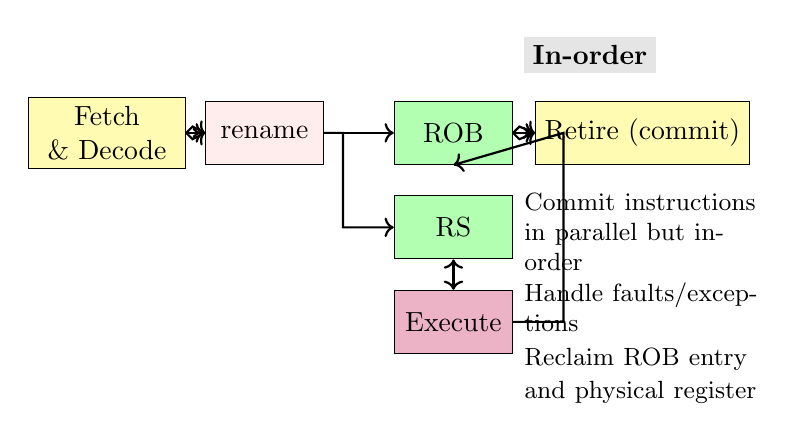
\begin{tikzpicture}[scale=0.8,
      block/.style={rectangle, draw, fill=yellow!30, minimum width=2cm, minimum height=0.8cm},
      rename/.style={rectangle, draw, fill=pink!30, minimum width=1.5cm, minimum height=0.8cm},
      pool/.style={rectangle, draw, fill=green!30, minimum width=1.5cm, minimum height=0.8cm},
      exe/.style={rectangle, draw, fill=purple!30, minimum width=1.5cm, minimum height=0.8cm},
      retire/.style={rectangle, draw, fill=yellow!30, minimum width=1.5cm, minimum height=0.8cm}]
      
      \node[block,align=center] (fetch) at (0,0) {Fetch \\\& Decode};
      \node[rename] (rename) at (2.5,0) {rename};
      \node[pool] (rob) at (5.5,0) {ROB};
      \node[pool] (rs) at (5.5,-1.5) {RS};
      \node[exe] (execute) at (5.5,-3) {Execute};
      \node[retire] (retire) at (8.5,0) {Retire (commit)};
      
      % Arrows
      \foreach \y in {-0.1, 0, 0.1} {
        \draw[->, thick] (fetch.east) -- ++(0.1,\y) -- (rename.west);
      }
      
      \draw[->, thick] (rename.east) -- (rob.west);
      \draw[->, thick] (rename.east) -- ++(0.3,0) -- ++(0,-1.5) -- (rs.west);
      
      % Bidirectional arrows between RS and Execute
      \draw[<->, thick] (rs.south) -- (execute.north);
      \draw[->, thick] (execute.east) -- ++(0.8,0) -- ++(0,3) -- (rob.south);
      
      % ROB to Retire
      \foreach \y in {-0.1, 0, 0.1} {
        \draw[->, thick] (rob.east) -- ++(0.1,\y) -- (retire.west);
      }
      
      % Annotations
      \node[text width=3cm, above] at (8.5,0.8) {\colorbox{gray!20}{\textbf{In-order}}};
      \node[text width=3cm, below] at (8.5,-0.8) {\small Commit instructions in parallel but in-order\\
        Handle faults/exceptions\\
        Reclaim ROB entry and physical register};
    \end{tikzpicture}
  \end{center}
\end{frame}


\begin{frame}{Large ROB and RS are Important}
  \begin{itemize}
    \item \textbf{A Large RS}
    \begin{itemize}
      \item Increase the window in which looking for independent instructions
      \begin{itemize}
        \item Exposes more parallelism potential
      \end{itemize}
    \end{itemize}
    
    \item \textbf{Large ROB}
    \begin{itemize}
      \item The ROB is a superset of the RS $\Rightarrow$ ROB size $\geq$ RS size
      \item Allows for covering long latency operations (cache miss, divide)
    \end{itemize}
    
    \item \textbf{Example}
    \begin{itemize}
      \item Assume there is a Load that misses the L1 cache and hits the L2 cache
      \begin{itemize}
        \item Data takes $\sim$10 cycles to return $\Rightarrow$ $\sim$30 new instrs get into pipeline
      \end{itemize}
      \item Instructions following the Load cannot commit $\Rightarrow$ pile up in the ROB
      \item Instructions independent of the load are executed, and leave the RS
      \begin{itemize}
        \item As long as the ROB is not full, we can keep fetching, renaming, and executing instructions
      \end{itemize}
    \end{itemize}
  \end{itemize}
\end{frame}

\begin{frame}{Out Of Order Execution Summary}
  \begin{itemize}
    \item \textbf{Look ahead in a window of instructions}
    \begin{itemize}
      \item Dispatch \emph{ready instructions} to execution
      \begin{itemize}
        \item Do not depend on data from previous instructions still not executed
        \item Have the required execution resources available
      \end{itemize}
    \end{itemize}
    
    \item \textbf{Advantages}
    \begin{itemize}
      \item Exploit Instruction Level Parallelism beyond adjacent instructions
      \item Help cover latencies (e.g., L1 data cache miss, divide)
      \item Superior/complementary to compiler scheduler
      \begin{itemize}
        \item Can look for ILP beyond conditional branches
        \item In a given control path instructions may be independent
        \item Register Renaming: use more than the number architectural registers
      \end{itemize}
    \end{itemize}
    
    \item \textbf{Complex micro-architecture}
    \begin{itemize}
      \item Register renaming, complex scheduler, misprediction recovery
      \item Memory ordering (coming next)
    \end{itemize}
  \end{itemize}
\end{frame}

\begin{frame}
  \begin{center}
    \vspace{3cm}
    {\Huge \textbf{OOO Execution of Memory Operations}}
  \end{center}
\end{frame}

\begin{frame}{OOO Execution of Memory Operations}
  \begin{itemize}
    \item \textbf{The RS dispatches instructions based on \textcolor{green}{register} dependencies}
    \begin{itemize}
      \item The RS cannot detect \textcolor{purple}{memory} dependencies
      \begin{center}
        \texttt{store Mem[r1+r3*2] $\leftarrow$ r9}\\
        \texttt{load  r2 $\leftarrow$ Mem[r10+r7*2]}
      \end{center}
      \begin{itemize}
        \item Does not know the load/store memory addresses
      \end{itemize}
      
      \item The RS dispatches load/store instructions to the Address Generation Unit (AGU) when the sources for the address calculation are ready
      
      \item The AGU calculates the virtual memory address:
      \begin{center}
        \colorbox{gray!20}{Base Register + (Scale × Index Register) + Displacement}
      \end{center}
    \end{itemize}
    
    \item \textbf{The AGU sends the address to the Memory Order Buffer (MOB)}
    \begin{itemize}
      \item The MOB resolves memory dependencies and enforces memory ordering
    \end{itemize}
  \end{itemize}
\end{frame}

\begin{frame}{Load/Store Ordering}
  \begin{itemize}
    \item \textbf{Loads can be executed OOO with respect to other loads}
    \begin{itemize}
      \item Not allowing this would have a very big performance impact
    \end{itemize}
    
    \item \textbf{Stores write value to the data-cache in-order, post retirement}
    \begin{itemize}
      \item Stores cannot write values to the data-cache speculatively
      \begin{itemize}
        \item There is no simple way to undo them
      \end{itemize}
      \item Stores to the data-cache are never re-ordered among themselves
      \begin{itemize}
        \item Must be seen in-order to other cores or agents
      \end{itemize}
    \end{itemize}
    
    \item \textbf{Loads need to maintain correct order with respect to stores}
    \begin{itemize}
      \item The RS dispatches instructions based on \textcolor{gray}{register dependencies}
      \begin{itemize}
        \item The RS cannot detect memory dependencies
      \end{itemize}
      \item The MOB tracks dependencies between loads and stores
    \end{itemize}
  \end{itemize}
\end{frame}

\begin{frame}{Load/Store Ordering}
    The MOB tracks dependencies between loads and stores
    \begin{block}{An older Store has an unresolved address $\rightarrow$ block Load}
      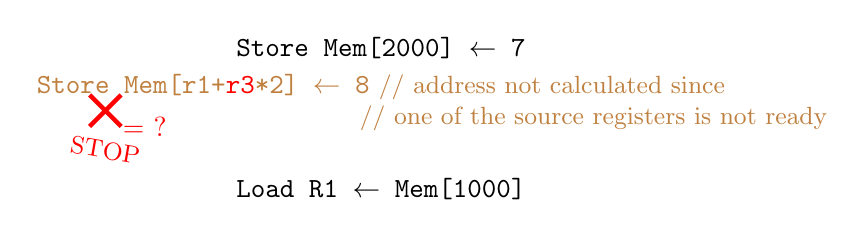
\begin{tikzpicture}[remember picture]
        \node[align=left] at (4,1.5) {\texttt{Store Mem[2000] $\leftarrow$ 7}};
        \node[align=left, brown] at (4,1) {\texttt{Store Mem[r1+\tikzmark{r3}\textcolor{red}{r3}*2] $\leftarrow$ 8} \small // address not calculated since};
        \node[align=left, brown] at (6.7,0.6) {\small // one of the source registers is not ready};
        \node[red] at (1,0.5) {= ?};
        \draw[red, ultra thick] (0.3,0.5) -- (0.7,0.9);
        \draw[red, ultra thick] (0.3,0.9) -- (0.7,0.5);
        \node[red, rotate=-10] at (0.5,0.2) {\small STOP};
        \node[align=left] at (4,-0.3) {\texttt{Load R1 $\leftarrow$ Mem[\tikzmark{target}1000]}};
      \end{tikzpicture}
      \begin{tikzpicture}[remember picture, overlay]
        \draw[->, red, thick] ([xshift=4pt,yshift=-1pt]pic cs:r3) -- ([xshift=5,yshift=12pt]pic cs:target);
      \end{tikzpicture}
    \end{block}
    \begin{block}{Older Store to same address, but Store's data \underline{is not ready} $\rightarrow$ block Load}
    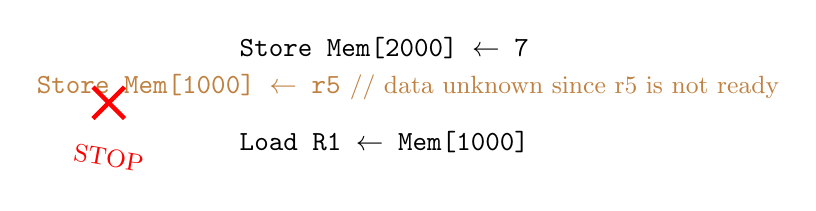
\begin{tikzpicture}
      \node[align=left] at (4,1.2) {\texttt{Store Mem[2000] $\leftarrow$ 7}};
      \node[align=left, brown] at (4.3,0.7) {\texttt{Store Mem[1000] $\leftarrow$ r5} \small // data unknown since r5 is not ready};
      \draw[red, ultra thick] (0.3,0.3) -- (0.7,0.7);
      \draw[red, ultra thick] (0.3,0.7) -- (0.7,0.3);
      \node[red, rotate=-10] at (0.5,-0.2) {\small STOP};
      \node[align=left] at (4,0) {\texttt{Load R1 $\leftarrow$ Mem[1000]}};
    \end{tikzpicture}
    \end{block}
\end{frame}

\begin{frame}{Store Implemented as 2 $\mu$ops}
  \begin{itemize}
    \item \textbf{Stores are decoded into two independent $\mu$ops}
    \begin{itemize}
      \item STA (store-address): calculates the address of the store
      \item STD (store-data): stores the data into the Store Data buffer
      \begin{itemize}
        \item This makes the data available to any Load that needs it
        \item The actual write to memory is done when the store retires
      \end{itemize}
    \end{itemize}
    
    \vspace{0.5cm}
    
    \item \textbf{Separating Store to STA \& STD improves performance}
    \begin{itemize}
      \item Allows STA to dispatch earlier, even before the data is known
      \begin{itemize}
        \item Address conflicts resolved earlier $\Rightarrow$\\
        opens memory pipeline for other loads
      \end{itemize}
      
      \item STA and STD can be issued to execution units in parallel
      \begin{itemize}
        \item STA dispatched to AGU when its sources (base + index) are ready
        \item STD dispatched to SDB when its source operand is available
      \end{itemize}
    \end{itemize}
  \end{itemize}
\end{frame}


\begin{frame}{Memory Order Buffer (MOB)}
  \begin{columns}
    \begin{column}{0.7\textwidth}
      \begin{itemize}
        \item \textbf{Store Coloring}
        \begin{itemize}
          \item Stores: track in \emph{Store Buffer} $\rightarrow$ alloc \textbf{SBID}
          \item Loads: track in \emph{Load Buffer} $\rightarrow$ alloc \textbf{LBID}, save \textbf{SBID}
          \item In-order allocation
        \end{itemize}
        
        \item \textbf{Loads check against prior stores}
        \begin{itemize}
          \item Those with SBID $\leq$ load's SBID
        \end{itemize}
        
        \item \textbf{Load blocks when:}
        \begin{itemize}
          \item Relevant STA has unresolved address
          \item STA to same address awaits data
          \item Data cache misses
        \end{itemize}
        
        \item \textbf{MOB handles blocked loads:}
        \begin{itemize}
          \item Records blocking info in Load Buffer
          \item Re-dispatches on wake-up signal
          \item May block again on new condition
        \end{itemize}
        
        \item \textbf{Unblocked loads → execute (bypass)}
      \end{itemize}
    \end{column}
    
    \begin{column}{0.3\textwidth}
      \begin{center}
        \begin{tabular}{|c|c|c|}
          \hline
          & \textbf{LBID} & \textbf{SBID} \\
          \hline
          \rowcolor{blue!15} Store & - & 0 \\
          \hline
          \rowcolor{green!15} Store & - & 1 \\
          \hline
          \rowcolor{green!15} Load & 0 & 1 \\
          \hline
          \rowcolor{orange!15} Store & - & 2 \\
          \hline
          \rowcolor{orange!15} Load & 1 & 2 \\
          \hline
          \rowcolor{orange!15} Load & 2 & 2 \\
          \hline
          \rowcolor{orange!15} Load & 3 & 2 \\
          \hline
          \rowcolor{red!15} Store & - & 3 \\
          \hline
          \rowcolor{red!15} Load & 4 & 3 \\
          \hline
        \end{tabular}
      \end{center}
    \end{column}
  \end{columns}
\end{frame}


% Updated macro with more flexibility and queue colors
\newcommand{\drawpipelineCustomExt}[9]{%
    % Parameters: 
    % #1: Predict/Fetch color (0=normal, 1=highlight, 2=gray)
    % #2: Decode color
    % #3: Alloc color  
    % #4: Schedule/EX color
    % #5: Retire color
    % #6: IQ queue color (0=green, 1=gray, 2=half gray/half green)
    % #7: uopq queue color (0=green, 1=gray, 2=half gray/half green)
    % #8: RS queue color (0=green, 1=gray, 2=half gray/half green)
    % #9: ROB queue color (0=green, 1=gray, 2=half gray/half green)
    \begin{tikzpicture}[
        remember picture,
        stage/.style={rectangle, draw=black, thick, minimum width=2.2cm, minimum height=0.9cm, font=\footnotesize, fill=orange!40},
        stageHighlight/.style={stage, fill=yellow!60},
        stageGray/.style={stage, fill=gray!30},
        queue/.style={rectangle, draw=black, fill=green!60, minimum width=0.15cm, minimum height=0.7cm},
        queueGray/.style={rectangle, draw=black, fill=gray!30, minimum width=0.15cm, minimum height=0.7cm},
        scale=0.75, transform shape
    ]
        
        % Predict/Fetch
        \ifnum#1=1
            \node[stageHighlight] (fetch) {Predict/Fetch};
        \else
            \ifnum#1=2
                \node[stageGray] (fetch) {Predict/Fetch};
            \else
                \node[stage] (fetch) {Predict/Fetch};
            \fi
        \fi
        
        % IQ queue
        \ifnum#6=1
            \node[queueGray, right=0.1cm of fetch] (iq1) {};
            \node[queueGray, right=0 of iq1] (iq2) {};
            \node[queueGray, right=0 of iq2] (iq3) {};
            \node[queueGray, right=0 of iq3] (iq4) {};
        \else
            \ifnum#6=2
                \node[queueGray, right=0.1cm of fetch] (iq1) {};
                \node[queueGray, right=0 of iq1] (iq2) {};
                \node[queue, right=0 of iq2] (iq3) {};
                \node[queue, right=0 of iq3] (iq4) {};
            \else
                \node[queue, right=0.1cm of fetch] (iq1) {};
                \node[queue, right=0 of iq1] (iq2) {};
                \node[queue, right=0 of iq2] (iq3) {};
                \node[queue, right=0 of iq3] (iq4) {};
            \fi
        \fi
        
        % Decode
        \ifnum#2=1
            \node[stageHighlight, right=0.1cm of iq4] (decode) {Decode};
        \else
            \ifnum#2=2
                \node[stageGray, right=0.1cm of iq4] (decode) {Decode};
            \else
                \node[stage, right=0.1cm of iq4] (decode) {Decode};
            \fi
        \fi
        
        % uopq queue
        \ifnum#7=1
            \node[queueGray, right=0.1cm of decode] (uopq1) {};
            \node[queueGray, right=0 of uopq1] (uopq2) {};
            \node[queueGray, right=0 of uopq2] (uopq3) {};
            \node[queueGray, right=0 of uopq3] (uopq4) {};
        \else
            \ifnum#7=2
                \node[queueGray, right=0.1cm of decode] (uopq1) {};
                \node[queueGray, right=0 of uopq1] (uopq2) {};
                \node[queue, right=0 of uopq2] (uopq3) {};
                \node[queue, right=0 of uopq3] (uopq4) {};
            \else
                \node[queue, right=0.1cm of decode] (uopq1) {};
                \node[queue, right=0 of uopq1] (uopq2) {};
                \node[queue, right=0 of uopq2] (uopq3) {};
                \node[queue, right=0 of uopq3] (uopq4) {};
            \fi
        \fi
        
        % Alloc
        \ifnum#3=1
            \node[stageHighlight, right=0.1cm of uopq4, minimum width=1.5cm] (alloc) {Alloc};
        \else
            \ifnum#3=2
                \node[stageGray, right=0.1cm of uopq4, minimum width=1.5cm] (alloc) {Alloc};
            \else
                \node[stage, right=0.1cm of uopq4, minimum width=1.5cm] (alloc) {Alloc};
            \fi
        \fi
        
        % RS queue
        \ifnum#8=1
            \node[queueGray, right=0.1cm of alloc] (rs1) {};
            \node[queueGray, right=0 of rs1] (rs2) {};
            \node[queueGray, right=0 of rs2] (rs3) {};
            \node[queueGray, right=0 of rs3] (rs4) {};
        \else
            \ifnum#8=2
                \node[queueGray, right=0.1cm of alloc] (rs1) {};
                \node[queueGray, right=0 of rs1] (rs2) {};
                \node[queue, right=0 of rs2] (rs3) {};
                \node[queue, right=0 of rs3] (rs4) {};
            \else
                \node[queue, right=0.1cm of alloc] (rs1) {};
                \node[queue, right=0 of rs1] (rs2) {};
                \node[queue, right=0 of rs2] (rs3) {};
                \node[queue, right=0 of rs3] (rs4) {};
            \fi
        \fi
        
        % Schedule/EX
        \ifnum#4=1
            \node[stageHighlight, right=0.1cm of rs4, minimum width=1.8cm] (schedule) {Schedule};
            \node[stageHighlight, right=0 of schedule, minimum width=0.8cm] (ex) {JEU};
        \else
            \ifnum#4=2
                \node[stageGray, right=0.1cm of rs4, minimum width=1.8cm] (schedule) {Schedule};
                \node[stageGray, right=0 of schedule, minimum width=0.8cm] (ex) {EX};
            \else
                \node[stage, right=0.1cm of rs4, minimum width=1.8cm] (schedule) {Schedule};
                \node[stage, right=0 of schedule, minimum width=0.8cm] (ex) {EX};
            \fi
        \fi
        
        % ROB queue (shortened to 4 entries)
        \ifnum#9=1
            \node[queueGray, right=0.1cm of ex] (rob1) {};
            \node[queueGray, right=0 of rob1] (rob2) {};
            \node[queueGray, right=0 of rob2] (rob3) {};
            \node[queueGray, right=0 of rob3] (rob4) {};
        \else
            \ifnum#9=2
                \node[queueGray, right=0.1cm of ex] (rob1) {};
                \node[queueGray, right=0 of rob1] (rob2) {};
                \node[queue, right=0 of rob2] (rob3) {};
                \node[queue, right=0 of rob3] (rob4) {};
            \else
                \node[queue, right=0.1cm of ex] (rob1) {};
                \node[queue, right=0 of rob1] (rob2) {};
                \node[queue, right=0 of rob2] (rob3) {};
                \node[queue, right=0 of rob3] (rob4) {};
            \fi
        \fi
        
        % Retire
        \ifnum#5=1
            \node[stageHighlight, right=0.1cm of rob4] (retire) {Retire};
        \else
            \ifnum#5=2
                \node[stageGray, right=0.1cm of rob4] (retire) {Retire};
            \else
                \node[stage, right=0.1cm of rob4] (retire) {Retire};
            \fi
        \fi
        
        % Labels for queues
        \node[font=\scriptsize] at ($(iq1.south)!0.5!(iq4.south)+(0,-0.15)$) {IQ};
        \node[font=\scriptsize] at ($(uopq1.south)!0.5!(uopq4.south)+(0,-0.15)$) {$\mu$opq};
        \node[font=\scriptsize] at ($(rs1.south)!0.5!(rs4.south)+(0,-0.15)$) {RS};
        \node[font=\scriptsize] at ($(rob1.south)!0.5!(rob4.south)+(0,-0.15)$) {ROB};
    \end{tikzpicture}
}

% Original macro for backward compatibility - just calls extended version with all queues green
\newcommand{\drawpipelineCustom}[5]{%
    \drawpipelineCustomExt{#1}{#2}{#3}{#4}{#5}{0}{0}{0}{0}%
}

% Simplified version for basic highlighting
\newcommand{\drawpipeline}[1]{%
    \ifnum#1=0
        \drawpipelineCustom{0}{0}{0}{0}{0}
    \else
        \ifnum#1=1
            \drawpipelineCustom{1}{0}{0}{0}{0}
        \else
            \ifnum#1=2
                \drawpipelineCustom{0}{1}{0}{0}{0}
            \else
                \ifnum#1=3
                    \drawpipelineCustom{0}{0}{1}{0}{0}
                \else
                    \ifnum#1=4
                        \drawpipelineCustom{0}{0}{0}{1}{0}
                    \else
                        \ifnum#1=5
                            \drawpipelineCustom{0}{0}{0}{0}{1}
                        \fi
                    \fi
                \fi
            \fi
        \fi
    \fi
}


% Slide 1: OOO Machine Pipeline
\begin{frame}{OOO Machine Pipeline}
    \centering
    
    % Background areas for Frontend/Backend
    \begin{tikzpicture}[overlay, remember picture]
        % Define coordinates for the rectangles
        \coordinate (frontend-tl) at ($(current page.center)+(-7.5,3)$);
        \coordinate (frontend-br) at ($(current page.center)+(-0.5,1)$);
        \coordinate (backend-tl) at ($(current page.center)+(-0.5,3)$);
        \coordinate (backend-br) at ($(current page.center)+(7.5,1)$);
        
        % Frontend background (left side)
        \fill[cyan!10, rounded corners=5pt] 
            (frontend-tl) rectangle (frontend-br);
        % Backend background (right side)
        \fill[orange!10, rounded corners=5pt] 
            (backend-tl) rectangle (backend-br);
        
        % Category labels positioned relative to rectangle bottoms
        \node[font=\footnotesize\sffamily\itshape, text=cyan!60!black] 
            at ($(frontend-tl)!0.5!(frontend-br)+(0,-0.3)$) {Frontend};
        \node[font=\footnotesize\sffamily\itshape, text=orange!60!black] 
            at ($(backend-tl)!0.5!(backend-br)+(0,-0.3)$) {Backend};
    \end{tikzpicture}
    
    \drawpipeline{0}
    \begin{itemize}
    \item \textbf{IQ -- Instruction Queue}
    \begin{itemize}
        \item Used mostly in variable length instructions architectures
        \item Smooth the variable number of instruction from a given fetch line
    \end{itemize}
    
    \item \textbf{$\mu$opq}
    \begin{itemize}
        \item Buffer between the fronted and the backend of the machine
        \item Frontend oversupply periods may cover for frontend undersupply periods
    \end{itemize}
    
    \item \textbf{Buffers may be bypassed -- depending on implementation}
    \begin{itemize}
        \item If bypassed, don't cost a cycle when the buffer is empty, e.g., after pipeline flush due to jump misprediction, or following a period of undersupply
    \end{itemize}
  \end{itemize}
\end{frame}

% Slide 2: Pipeline: Predict/Fetch (already provided by user)
\begin{frame}{Pipeline: Predict/Fetch}
    \centering
    \drawpipeline{1}
    
    \vspace{0.5cm}
    \begin{columns}[T]
        \begin{column}{0.9\textwidth}
            \begin{itemize}
                \item Predict the next fetch line
                \item Fetch multiple instruction bytes from the I\$
                \item In case of a variable instruction length architecture (like x86)
                \begin{itemize}
                    \item Length-decode instructions within the fetched instruction bytes
                    \item Write the instructions into an Instruction Queue
                \end{itemize}
            \end{itemize}
        \end{column}
    \end{columns}
\end{frame}

% Slide 3: Pipeline: Decode
\begin{frame}{Pipeline: Decode}
    \centering
    \drawpipeline{2}
    
    \vspace{0.5cm}
    \begin{columns}[T]
        \begin{column}{0.9\textwidth}
            \begin{itemize}
                \item Read multiple instructions from the IQ
                \item Decode the instructions
                \begin{itemize}
                    \item For x86 processors, each instruction is decoded into $\geq$1 $\mu$ops
                    \item $\mu$ops are RISC-like instructions
                \end{itemize}
                \item Write the resulting $\mu$ops into the Instruction Decoder Queue ($\mu$opq)
            \end{itemize}
        \end{column}
    \end{columns}
\end{frame}

% Slide 4: Pipeline: Allocate/Rename
\begin{frame}{Pipeline: Allocate/Rename}
    \centering
    \drawpipeline{3}
    
    \vspace{0.5cm}
    \begin{columns}[T]
        \begin{column}{0.9\textwidth}
            \begin{itemize}
                \item Rename multiple $\mu$ops
                \item Perform port-binding per $\mu$op
                \begin{itemize}
                    \item Select the execution port to which the $\mu$op is dispatched when ready
                \end{itemize}
                \item Allocate ROB/RS entry per $\mu$op
                \begin{itemize}
                    \item If source data is available from ROB or ARF, write data to RS
                    \item Otherwise, mark data not ready in RS
                \end{itemize}
            \end{itemize}
        \end{column}
    \end{columns}
\end{frame}

% Slide 5: Pipeline: EXE
\begin{frame}{Pipeline: EXE}
    \centering
    \drawpipeline{4}
    
    \vspace{0.5cm}
    \begin{columns}[T]
        \begin{column}{0.9\textwidth}
            \textbf{Ready/Schedule}
            \begin{itemize}
                \item Check for data-ready $\mu$ops if the needed port / functional unit are available
                \item Select and dispatch multiple ready $\mu$ops/clock to EXE
            \end{itemize}
            
            \textbf{Write back results into RS/ROB}
            \begin{itemize}
                \item Wake-up $\mu$ops in the RS that are waiting for the results as sources
                \begin{itemize}
                    \item Update data-ready status of these $\mu$ops in the RS
                \end{itemize}
                \item Write back results into the Physical Registers
                \item Reclaim RS entries
            \end{itemize}
        \end{column}
    \end{columns}
\end{frame}

% Slide 6: Pipeline: Retire
\begin{frame}{Pipeline: Retire}
    \centering
    \drawpipeline{5}
    
    \vspace{0.5cm}
    \begin{columns}[T]
        \begin{column}{0.9\textwidth}
            \textbf{Retire oldest $\mu$ops in the ROB}
            \begin{itemize}
                \item A $\mu$op may retire if
                \begin{itemize}
                    \item Its ``executed'' bit is set
                    \item It is not marked with an exception / fault
                    \item All preceding $\mu$ops are eligible for retirement
                \end{itemize}
                \item Commit results from the Physical Register to the Arch Register
                \item Reclaim the ROB entry
            \end{itemize}
            
            \textbf{In case of exception / fault}
            \begin{itemize}
                \item Flush the pipeline and handle the exception / fault
                \item Restart the program
            \end{itemize}
        \end{column}
    \end{columns}
\end{frame}

% Slide 7: Jump Misprediction - Flush at Retire
\begin{frame}{Jump Misprediction -- Flush at Retire}
    \centering
    
    \begin{columns}[T]
        \begin{column}{0.9\textwidth}
            \textbf{When a mispredicted jump retires}
            \begin{itemize}
                \item Flush the pipeline
                \begin{itemize}
                    \item When the jump commits, all the instructions remaining in the pipe are younger than the jump $\Rightarrow$ from the wrong path
                \end{itemize}
                \item Reset the renaming map
                \begin{itemize}
                    \item So all the registers are mapped to the architectural registers
                    \item This is ok since there are no consumers of physical registers (pipe is flushed)
                \end{itemize}
                \item Start fetching instructions from the correct path
            \end{itemize}
            
            \vspace{0.3cm}
            \textbf{Disadvantage}
            \begin{itemize}
                \item Very high misprediction penalty
                \item Misprediction is already known after the jump was executed
                \item We will see ways to recover a misprediction at execution
            \end{itemize}
        \end{column}
    \end{columns}
\end{frame}

% Slide 8: Flush at Retire: Misp. Jump at EXE
\begin{frame}{Flush at Retire: Misp. Jump at EXE}
    \centering
    \drawpipelineCustom{0}{0}{0}{1}{0}
    
    % Add Clear arrow from retire to alloc
    \begin{tikzpicture}[overlay, remember picture]
        % Arrow from retire to alloc showing what gets cleared when jump retires
        \coordinate (clear-start) at ($(retire.south)+(0,-0.3)$);
        \coordinate (clear-end) at ($(alloc.south)+(0,-0.3)$);
        
        % Draw the clear indication
        \draw[<->, red, thick] (clear-start) -- (clear-end);
        \node[red, font=\small\bfseries] at ($(clear-start)!0.5!(clear-end)+(0,-0.2)$) {Clear when jump retires};
    \end{tikzpicture}
    
    \vspace{0.5cm}
    \begin{columns}[T]
        \begin{column}{0.9\textwidth}
            \begin{itemize}
                \item \textbf{Misprediction detected when jump is executed}
                \begin{itemize}
                    \item Mark the jump as mispredicted in ROB
                \end{itemize}
            \end{itemize}
        \end{column}
    \end{columns}
\end{frame}

% Slide 9: Flush at Retire: Misp. Jump Retires
\begin{frame}{Flush at Retire: Misp. Jump Retires}
    \vspace{1cm}
    \centering
    \drawpipelineCustom{2}{2}{2}{2}{2}
    
    % Add flush arrow and text using node positions from the macro
    \begin{tikzpicture}[overlay, remember picture]
        \draw[->, red, ultra thick] (retire.north) -- ++(0,0.8) -| 
          node[red, font=\bfseries\small, below, near start] {Clear} (fetch.north)
          node[black, font=\scriptsize, near end, left, align=right] {Redirect Fetch\\+ update BPU};
    \end{tikzpicture}
    
    %\vspace{0.5cm}
    %\textbf{When the mispredicted jump retires}
    \begin{itemize}
        \item[]\textbf{When the mispredicted jump retires}
        \item All instructions in the pipe are younger than the jump \\
        $\Rightarrow$ all are from the wrong path $\Rightarrow$ flush the entire pipeline
        \item Reset the renaming map
        \begin{itemize}
            \item Map all the registers to the architectural registers
            \item This is ok since there are no consumers of physical registers (pipe is flushed)
        \end{itemize}
        \item Start fetching instructions from the correct path
    \end{itemize}
\end{frame}

% Slide 10: Jump Misprediction - Flush at Execute
\begin{frame}{Jump Misprediction -- Flush at Execute}
    \begin{itemize}
        \item[] \textbf{When a jump misprediction is detected (at jump execution)}
        \item Flush the in-order front-end
        \item Continue executing instructions already in the OOO part
        \begin{itemize}
            \item Including wrong-path instructions (waste of execution resources and power)
        \end{itemize}
        \item Start fetching and decoding instructions from the correct path
        \begin{itemize}
            \item Note that the ``correct'' path may still be wrong...
            \item An older instruction may cause an exception when it retires
            \item An older jump executed out-of-order can also mispredict
        \end{itemize}
        \item Block younger jumps (executed OOO) from clearing
        \item Stall the correct instruction stream at the Renamer
        \begin{itemize}
            \item The RAT (Register Alias Table) was wrongly updated by wrong-path instructions
        \end{itemize}
        \vspace{0.5cm}
        \item[] \textbf{When the mispredicted jump retires}
        \item Flush all instructions from the RS/ROB
        \begin{itemize}
            \item All are from the wrong path at this point
        \end{itemize}
        \item Reset the Renamer to point only to architectural registers
        \item Un-stall the Renamer and allow instructions from correct path to rename/allocate
    \end{itemize}
\end{frame}

% Slide 11: Flush at EXE: Jump Gets to EXE (first)
\begin{frame}{Flush at EXE: Jump Gets to EXE}
    \centering
    \drawpipelineCustom{0}{0}{0}{1}{0}
    
    \vspace{4cm} % Space for potential diagram
\end{frame}

% Slide 12: Flush at EXE: Jump Gets to EXE (detailed)
\begin{frame}{Flush at EXE : Jump Gets to EXE}
    \vspace{1cm}
    \centering
    \drawpipelineCustom{2}{2}{0}{1}{0}
    
    % Add Flush arrow and labels
    \begin{tikzpicture}[overlay, remember picture]
        \draw[->, red, ultra thick] (ex.north) -- ++(0,0.8) -| 
          node[red, font=\bfseries\small, below, near start] {Flush} (fetch.north)
          node[black, font=\scriptsize, near end, left, align=right] {Redirect Fetch\\+ update BPU};
        % draw red line left of alloc
        \draw[red, ultra thick] ([yshift=-1mm]alloc.south west) -- ([yshift=1mm]alloc.north west);
    \end{tikzpicture}
    
    \vspace{0.5cm}
    \begin{itemize}
        \item Flush the front-end and re-steer it to correct path
        \item Renamer state updated by wrong path $\Rightarrow$ Block further allocation
        \item Update BPU
        \item OOO not flushed
        \begin{itemize}
            \item Contains both instruction older and younger than the mispredicted jump
            \item Instructions already in the OOO part continue to execute
            \begin{itemize}
                \item Including wrong-path instructions (waste of execution resource and power)
            \end{itemize}
        \end{itemize}
        \item Block younger jumps from clearing
    \end{itemize}
\end{frame}

% Slide 13: Flush at EXE: Misp. Jump Retires
\begin{frame}{Flush at EXE : Misp. Jump Retires}
    \centering
    \vspace{1cm}
    \drawpipelineCustomExt{0}{0}{2}{2}{2}{1}{0}{0}{0}

    % Clear arrow
    \begin{tikzpicture}[overlay, remember picture]
        \draw[->, red, ultra thick] 
          (retire.north) -- ++(0,0.8) -| node[red, font=\bfseries\small, below, near start] {Clear} (alloc.north);
    \end{tikzpicture}
    
    \vspace{0.5cm}
    \begin{itemize}
        \item[] \textbf{When the mispredicted jump retires}
        \item Flush OOO
        \begin{itemize}
            \item Only instruction following the jump are left in the machine \\
            $\Rightarrow$ they must all be flushed
            \item Resets all state in the OOO (Renamer, RS, ROB, MOB, etc.)
            \item Reset the Renamer to point only to architectural registers, and unblock rename
        \end{itemize}
        \item Allow allocation of instructions from correct path
    \end{itemize}
\end{frame}

% Slide 14: Periodic Checkpoints
\begin{frame}{Periodic Checkpoints}
  \begin{columns}[T] % [T] aligns columns at the top
    % --- Left column: text (0.8\textwidth) ---
    \begin{column}{0.8\textwidth}
      \begin{itemize}
        \item \textbf{Allow allocation and execution of instructions from the correct path before the mispredicted jump retires}
        
        \vspace{0.3cm}
        \item \textbf{Every few instructions take a checkpoint of the Renamer}
        \begin{itemize}
          \item A snapshot of the current renaming map
          \item Taking a snapshot on every jump is expensive
        \end{itemize}
        
        \vspace{0.3cm}
        \item \textbf{In case of misprediction}
        \begin{itemize}
          \item Flush the frontend and start fetching instructions from the correct path
          \item Selectively flush younger instructions from the ROB/RS
          \item Recover Renamer to latest checkpoint taken prior to the mispredicted jump
          \item Recover Renamer to its state at the jump
          \begin{itemize}
            \item Rename instructions from the checkpoint and until the jump
          \end{itemize}
          \item Allow instructions from the correct path to allocate
        \end{itemize}
      \end{itemize}
    \end{column}

    % --- Right column: illustration (0.2\textwidth) ---
    \begin{column}{0.2\textwidth}
      \centering
      \textit{[Checkpoint illustration goes here]}
      % Example if you later add a figure:
      % \includegraphics[width=\linewidth]{checkpoint.pdf}
    \end{column}
  \end{columns}
\end{frame}

% Slide 15: Checkpoints: Jump Gets to EXE (first)
\begin{frame}{Checkpoints: Jump Gets to EXE}
    \centering
    \drawpipelineCustomExt{0}{0}{0}{1}{0}{1}{1}{2}{2}
    
    \begin{tikzpicture}[overlay, remember picture]
        \draw[->, red, ultra thick] (ex.north) -- ++(0,0.8) -| 
          node[red, font=\bfseries\small, below, near start] {Clear} (fetch.north)
          node[black, font=\scriptsize, near end, left, align=right] {update BPU};
    \end{tikzpicture}
 
    \vspace{0.5cm}
    \begin{itemize}
        \item \textbf{Clear raised on mispredicted jump}
    \end{itemize}
\end{frame}

% Slide 16: Checkpoints: Jump Gets to EXE (detailed)
\begin{frame}{Checkpoints: Jump Gets to EXE}
    \centering
    \drawpipelineCustomExt{0}{0}{0}{1}{0}{1}{1}{2}{2}
    
    % Add BPU Update and Clear labels
    \begin{tikzpicture}[overlay, remember picture]
        \draw[->, red, ultra thick] (ex.north) -- ++(0,0.8) -| 
          node[red, font=\bfseries\small, below, near start] {Clear} (fetch.north)
          node[black, font=\scriptsize, near end, left, align=right] {update BPU};
    \end{tikzpicture}
    
    \vspace{0.5cm}
    \begin{columns}[T]
        \begin{column}{0.9\textwidth}
            \textbf{Clear raised on mispredicted jump}
            \begin{itemize}
                \item Flush frontend and re-steer it to the correct path
                \item \textcolor{orange}{Flush all younger instructions in OOO}
                \begin{itemize}
                    \item Based on age (ROBid) comparison
                \end{itemize}
                \item Update BPU
                \item Block further allocation until the Renamer mapping is recovered
            \end{itemize}
        \end{column}
    \end{columns}
\end{frame}

% Slide 17: Checkpoints: Renamer Recovery (first)
\begin{frame}{Checkpoints: Renamer Recovery}
    \vspace{1cm}
    \centering
    \drawpipelineCustomExt{2}{2}{2}{0}{0}{1}{1}{2}{2}

    \begin{tikzpicture}[overlay, remember picture]
        \draw[red, ultra thick] ([yshift=-1mm]alloc.south west) -- ([yshift=1mm]alloc.north west);
    \end{tikzpicture}
    
    \begin{itemize}
        \item Restore Renamer from latest check-point before the jump
        \item Recover Renamer to its states just after the jump
        \item Meanwhile front-end starts fetching and decoding instructions from the correct path
    \end{itemize}
\end{frame}

% Slide 18: Checkpoints: Renamer Recovery (second)
\begin{frame}{Checkpoints: Renamer Recovery}
    \centering
    \drawpipelineCustomExt{0}{0}{1}{0}{0}{0}{0}{2}{2}
    
    \vspace{0.5cm}
    \begin{itemize}
        \item \textbf{Once done restoring the Renamer}
        \begin{itemize}
            \item allow allocation of instructions from correct path
        \end{itemize}
    \end{itemize}
\end{frame}
\end{document}
